\chapter{Validación e probas}

Neste capítulo realizaremos o deseño das probas da nosa aplicación. As probas son experimentos cunha especificación determinada. Céntranse en probar un aspecto puntual do sistema, parten dunhas premisas (parámetros, situación, contexto, etc.) definidas a priori, e espérase delas unha resposta consistente. A correspondencia entre o estado ou resposta que se espera da proba e o resultado da súa realización determinan a validez do aspecto que están a probar.

Para probar a nosa aplicación recorreremos a dous métodos, cada un centrarase nun escenario concreto. Por unha parte, a libraría JUnit pon á nosa disposición unha serie de clases, deseñadas para lanzar probas contra pequenos métodos ou bloques de execución. Esta solución será de gran utilidade para validar as funcionalidades que versan sobre o Modelo, xa que o Modelo manipula grandes cantidades de datos que de xeito programático se poden comprobar facilmente.

Os tests en JUnit adoitan finalizar cunha sentencia assetEquals(), que recibe dous obxectos e comproba que sexa iguais para aceptar a proba. En caso contrario devolven un mensaxe de erro e a traza para axudar a solventalo. Para poder asumir que as probas funcionan, necesitamos algo co que comparar os nosos métodos. Nalgúns casos, imos botar man das prestacións da libraría Weka para verificar que o estado final dunha estrutura de datos é o esperado. Deste xeito, poderemos defender que o método funciona apoiándose en que os métodos de Weka co que o validamos xa foron probados previamente.

En base a isto, comezaremos os nosos test creando dous métodos estáticos nunha clase chamada ``ValidFileLoading.java''. Estos métodos son loadARFF(String resourcePath) e loadCSV(String resourcePath). Ambos serán usados de acordo á documentación sobre o seu uso para ler un ficheiro en formato ARFF ou CSV (respectivamente) e extraer del unha instancia de ComparableInstances. Deste xeito xa poderemos asumir como válido que as instancesComparable que devolven son as correctas, as que contén o ficheiro do cal lle pasamos a dirección.

\begin{lstlisting}
public class ValidFileLoading {

    public static ComparableInstances loadARFF(String resourcePath) {
        ComparableInstances comparableInstances = null;
        try {
            ArffLoader loaderARFF = new ArffLoader();
            loaderARFF.setFile(new File(resourcePath));
            comparableInstances = new ComparableInstances(loaderARFF.getDataSet());
        } catch (IOException ex) {
            Logger.getLogger(ValidFileLoading.class.getName()).log(Level.SEVERE, null, ex);
        }
        return comparableInstances;
    }

    public static ComparableInstances loadCSV(String resourcePath) {
        ComparableInstances comparableInstances = null;
        try {
            CSVLoader loaderCSV = new CSVLoader();
            loaderCSV.setSource(new File(resourcePath));
            comparableInstances = new ComparableInstances(loaderCSV.getDataSet());

        } catch (IOException ex) {
            Logger.getLogger(ValidFileLoading.class.getName()).log(Level.SEVERE, null, ex);
        }
        return comparableInstances;
    }

}
\end{lstlisting}

Tamén incluiremos no directorio dos filtros dous ficheiros compatibles con JDataMotion, que empregaremos para realizar as probas: ``213\_N3.csv'' (40 atributos e 3251 instancias) e ``example01.arff'' (1 atributo nominal e 30 numéricos, e 569 instancias)

Sen embargo, JUnit non nos facilita do mesmo xeito a validación de métodos que implican cambios directos na interface de usuario. Probas a nivel gráfico como comprobar que se visualizan correctamente os diagramas de dispersión son menos asequibles realizándoos mediante código ca por simple observación. É por isto que adoptaremos a avaliación heurística para aqueles casos nos que a usabilidade (apariencia intuitiva, sencillez, facilidade de uso, etc.) sexa un importante factor a validar.

A continuación percorreremos de novo todos os requisitos que describimos na análise, para asignarlle un test de proba e executalo mostrando os resultados.

\subsection{Requisitos funcionais}

\subsubsection*{RF01}
\begin{description}
\item[Título] \hfill
Importar arquivos con datos para o experimento
\item[Descrición] \hfill
A aplicación debe permitir cargar do sistema de arquivos un ficheiro que conteña unha secuencia de datos (nun formato axeitado segundo o RNF01) para ser utilizados no experimento.
\item[Importancia] \hfill
Esencial
\item[Tipo de proba] \hfill
Test implementado en JUnit.
\item[Nome do test] \hfill
TestRF01\_1 e TestRF01\_2
\item[Código fonte]
TestRF01\_1:
\begin{lstlisting}
public void test() {
        Modelo modelo = new Modelo();
        Vista vista = new Vista();
        vista.inicializar(modelo, false);
        Controlador.setDebug(true);
        String resource = "example01.arff";
        try {
            String pathEntrada = new URI(getClass().getResource(resource).toString()).getPath();
            ComparableInstances is1 = ValidFileLoading.loadARFF(pathEntrada);
            vista.getControlador().manexarEvento(Controlador.IMPORTAR_FICHEIRO, pathEntrada);
            ComparableInstances is2 = modelo.getComparableInstances();
            assertEquals(is1, is2);
        } catch (URISyntaxException ex) {
            Logger.getLogger(getClass().getName()).log(Level.SEVERE, null, ex);
        }
    }
\end{lstlisting}
TestRF01\_2:
\begin{lstlisting}
public void test() {
        Modelo modelo = new Modelo();
        Vista vista = new Vista();
        vista.inicializar(modelo, false);
        Controlador.setDebug(true);
        String resource = "213_N3.csv";
        try {
            String pathEntrada = new URI(getClass().getResource(resource).toString()).getPath();
            ComparableInstances is1 = ValidFileLoading.loadCSV(pathEntrada);
            vista.getControlador().manexarEvento(Controlador.IMPORTAR_FICHEIRO, pathEntrada);
            ComparableInstances is2 = modelo.getComparableInstances();
            assertEquals(is1, is2);
        } catch (URISyntaxException ex) {
            Logger.getLogger(getClass().getName()).log(Level.SEVERE, null, ex);
        }
    }
\end{lstlisting}
\item[Descrición]
Instáncianse un Modelo e unha vista, inicialízanse utilizando o parámetro visualizacion=false para bloquear a aparición da interface gráfica e actívase a depuración. Importamos o recurso ``example01.arff'' para TestRF01\_1 ou ``213\_N3.csv'' para TestRF01\_2, con axuda dos métodos de Weka nos que imos confiar, e almacenamos as instancias obtidas en ``is1''. A continuación lanzamos ao Controlador un evento de tipo IMPORTAR\_FICHEIRO e almacenamos as instancias do modelo en ``is2''. Por último, metemos ``is1'' e ``is2'' como parámetros do método assertEquals(Object expected, Object actual), e si ambos son iguais o RF01 quedará validado para formatos CSV e ARFF. A sobrescritura do método equals(Object o) dentro de ComparableInstances permitiralle ás instancias desta clase seren pasadas ao assertEquals.
\item[Resultado]
Correcto.
\end{description}

\subsubsection*{RF02}
\begin{description}
\item[Título] \hfill
Exportar datos
\item[Descrición] \hfill
A aplicación debe permitir almacenar nun arquivo o conxunto de datos do experimento actual (tendo en conta filtrados, modificacións, datos engadidos ou eliminados...). Os arquivos de saída deberán respectar o RNF01 en canto a formato de almacenamento.
\item[Importancia] \hfill
Esencial
\item[Tipo de proba] \hfill
Test implementado en JUnit.
\item[Nome do test] \hfill
TestRF02\_1 e TestRF02\_2
\item[Código fonte]
TestRF02\_1:
\begin{lstlisting}
public void test() {
        Modelo modelo = new Modelo();
        Vista vista = new Vista();
        vista.inicializar(modelo, false);
        Controlador.setDebug(true);
        String resource = "example01.arff";
        String tempSaida = "temp01.csv";
        try {
            String pathEntrada = new URI(getClass().getResource(resource).toString()).getPath();
            ComparableInstances is1 = ValidFileLoading.loadARFF(pathEntrada);
            modelo.setComparableInstances(new ComparableInstances(is1));
            String pathSaida = new URI(getClass().getResource(".").toString()).getPath() + tempSaida;
            vista.getControlador().manexarEvento(Controlador.EXPORTAR_FICHEIRO, new Object[]{"csv", pathSaida});
            ComparableInstances is2 = ValidFileLoading.loadCSV(pathSaida);
            is1.setRelationName("");
            is2.setRelationName("");
            assertEquals(is1, is2);
        } catch (URISyntaxException ex) {
            Logger.getLogger(getClass().getName()).log(Level.SEVERE, null, ex);
        }
    } 
\end{lstlisting}
TestRF02\_2:
\begin{lstlisting}
public void test() {
        Modelo modelo = new Modelo();
        Vista vista = new Vista();
        vista.inicializar(modelo, false);
        Controlador.setDebug(true);
        String resource = "213_N3.csv";
        String tempSaida = "temp01.arff";
        try {
            String pathEntrada = new URI(getClass().getResource(resource).toString()).getPath();
            ComparableInstances is1 = ValidFileLoading.loadCSV(pathEntrada);
            modelo.setComparableInstances(new ComparableInstances(is1));
            String pathSaida = new URI(getClass().getResource(".").toString()).getPath() + tempSaida;
            vista.getControlador().manexarEvento(Controlador.EXPORTAR_FICHEIRO, new Object[]{"arff", pathSaida});
            ComparableInstances is2 = ValidFileLoading.loadARFF(pathSaida);
						assertEquals(is1, is2);
        } catch (URISyntaxException ex) {
            Logger.getLogger(getClass().getName()).log(Level.SEVERE, null, ex);
        }
    }
\end{lstlisting}
\item[Descrición]
Instáncianse un Modelo e unha vista, inicialízanse utilizando o parámetro visualizacion=false para bloquear a aparición da interface gráfica e actívase a depuración. Importamos o recurso ``example01.arff'' para TestRF02\_1 ou ``213\_N3.csv'' para TestRF02\_2, con axuda dos métodos de Weka nos que imos confiar, e almacenamos as instancias obtidas en ``is1''. A continuación lanzamos ao Controlador un evento de tipo EXPORTAR\_FICHEIRO, pasándolle a dirección dun arquivo temporal en formato CSV para TestRF02\_1 ou en formato ARFF para TestRF02\_2. Despois disto, utilizamos as clases de importación nas que estamos confiando para obter as instancias dende o arquivo ao que acabamos de exportar e almacenamos o seu contido en ``is2''. Por último, metemos ``is1'' e ``is2'' como parámetros do método assertEquals(Object expected, Object actual), e si ambos son iguais o RF02 quedará validado para formatos CSV e ARFF. A sobrescritura do método equals(Object o) dentro de ComparableInstances permitiralle ás instancias desta clase seren pasadas ao assertEquals. En TestRF02\_1 debemos eliminar os nomes de relación das dúas ComparableInstances para ser xustos, xa que o arquivo ARFF perdeu o seu no proceso de exportación a CSV.
\item[Resultado]
Correcto.
\end{description}

\subsubsection*{RF03}
\begin{description}
\item[Título] \hfill
Gardar sesión
\item[Descrición] \hfill
A aplicación debe permitir gardar en disco a sesión (ou experimento) actual tal e como está no momento de executar esta acción.
\item[Importancia] \hfill
Esencial
\item[Tipo de proba] \hfill
Test implementado en JUnit.
\item[Nome do test] \hfill
TestRF0304
\item[Código fonte]
\begin{lstlisting}
public void test() {
        Modelo modelo = new Modelo();
        Vista vista = new Vista();
        vista.inicializar(modelo, false);
        Controlador.setDebug(true);
        String resource = "example01.arff";
        String archivoSesion = "temp01.jdms";
        try {
            String pathEntrada = new URI(getClass().getResource(resource).toString()).getPath();
            ComparableInstances is1 = ValidFileLoading.loadARFF(pathEntrada);
            modelo.setComparableInstances(new ComparableInstances(is1));
            modelo.setDireccionAoFicheiro(pathEntrada);
            modelo.setHashCodeFicheiro(Modelo.resumirFicheiroSHA1(new File(pathEntrada)));
            String pathSaida = new URI(getClass().getResource(".").toString()).getPath() + archivoSesion;
            /* se modificamos un dato manualmente, a sesion non o rexistra
             e ao restaurar a sesion o arquivo segue sendo igual ao inicial */
            modelo.getComparableInstances().instance(5).setValue(5, 666);
            /* se lanzamos un comando, a sesión rexistrao e entonces a proba fallaria
             porque se volveria a executar o comando ao restaurar a sesion, e xa non seria igual ao inicial */
            //vista.getControlador().manexarEvento(Controlador.MUDAR_DATO, new Object[]{5, 5, 666});
            vista.getControlador().manexarEvento(Controlador.GARDAR_SESION, pathSaida);
            vista.getControlador().manexarEvento(Controlador.ABRIR_SESION, pathSaida);
            ComparableInstances is2 = modelo.getComparableInstances();
            assertEquals(is1, is2);
        } catch (Exception ex) {
            Logger.getLogger(TestRF0304.class.getName()).log(Level.SEVERE, null, ex);
        }
    }
\end{lstlisting}
\item[Descrición]
Tras inicializar o sistema do mesmo xeito ca en test anteriores, cárgase o ficheiro ``example01.arff'' en ``is1'' por medio de ValidFileLoading (importación confiable). Asígnase ao modelo unha copia das ComparableInstances obtidas, de xeito que ``is1'' siga referenciando as instancias orixinais. Tamén se asigna a dirección ao ficheiro e o seu hash, pois o Modelo compróbaos ao abrir unha sesión por motivos de consistencia. A continuación modifícanse directamente as instancias, sen axuda de eventos. Despois lanzamos un evento GARDAR\_SESION e outro ABRIR\_SESION, ambos coa mesma dirección. Almacenamos as instancias que temos agora en ``is2'', colocándoas ás dúas no assertEquals. A modificación manual non debería provocar o error da proba, pois foi creada manualmente e non por un comando, así que ao restaurar a sesión esta modificación non se repetirá. 
\item[Resultado]
Correcto.
\end{description}

\subsubsection*{RF04}
\begin{description}
\item[Título] \hfill
Abrir sesión
\item[Descrición] \hfill
A aplicación debe permitir restaurar unha sesión (ou experimento) gardada anteriormente, de xeito que se atope exactamente igual ca no momento en que se gardou.
\item[Importancia] \hfill
Esencial
\item[Tipo de proba] \hfill
Test implementado en JUnit.
\item[Nome do test] \hfill
TestRF0304 (xa mencionado).
\end{description}

\subsubsection*{RF05}
\begin{description}
\item[Título] \hfill
Representar os datos en forma de táboa
\item[Descrición] \hfill
A aplicación debe ser capaz de amosar os datos segundo unha táboa na que figuren cabeceiras, tipos, valores, etc.
\item[Importancia] \hfill
Esencial
\item[Tipo de proba] \hfill
Avaliación heurística
\item[Descrición]
Ao abrir un ficheiro de tipo ARFF ou CSV coa aplicación, aparece no menú Modelo toda a información que necesitamos.
\begin{figure}
\centering
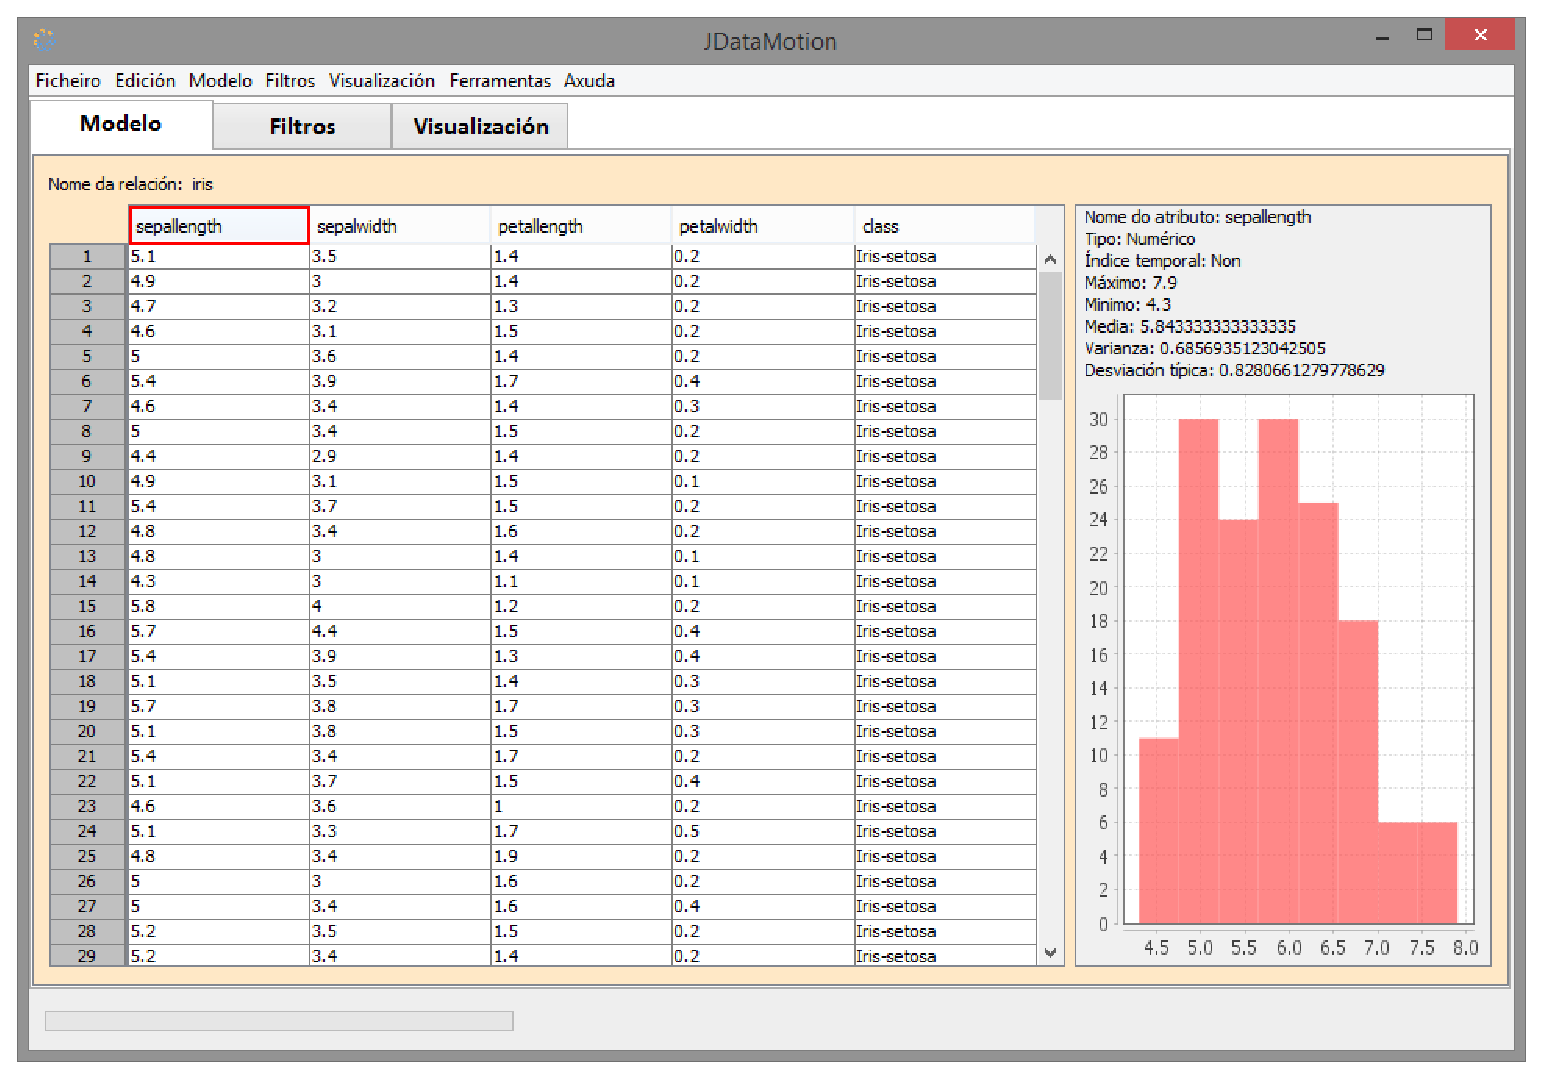
\includegraphics[width=\textwidth,height=\textheight,keepaspectratio]{figuras/RF05}
\caption{Comprobación heurística do RF05}
\label{RF05}
\end{figure}
\item[Resultado]
Correcto.
\end{description}

\subsubsection*{RF06}
\begin{description}
\item[Título] \hfill
Insertar datos no experimento actual
\item[Descrición] \hfill
A aplicación debe permitir a inserción dinámica de datos no experimento actual.
\item[Importancia] \hfill
Esencial
\item[Tipo de proba] \hfill
Test implementado en JUnit.
\item[Nome do test] \hfill
TestRF06\_1 e TestRF06\_2
\item[Código fonte]
TestRF06\_1:
\begin{lstlisting}
public void test() {
        Modelo modelo = new Modelo();
        Vista vista = new Vista();
        vista.inicializar(modelo, false);
        Controlador.setDebug(true);
        String resource = "example01.arff";
        try {
            String pathEntrada = new URI(getClass().getResource(resource).toString()).getPath();
            ComparableInstances is1 = ValidFileLoading.loadARFF(pathEntrada);
            modelo.setComparableInstances(new ComparableInstances(is1));
            vista.getControlador().manexarEvento(Controlador.ENGADIR_DATOS, null);
            is1.add(new DenseInstance(is1.numAttributes()));
            ComparableInstances is2 = modelo.getComparableInstances();
            assertEquals(is1, is2);
        } catch (URISyntaxException ex) {
            Logger.getLogger(getClass().getName()).log(Level.SEVERE, null, ex);
        }
    }
\end{lstlisting}
TestRF06\_2:
\begin{lstlisting}
public void test() {
        Modelo modelo = new Modelo();
        Vista vista = new Vista();
        vista.inicializar(modelo, false);
        Controlador.setDebug(true);
        String resource = "example01.arff";
        try {
            String pathEntrada = new URI(getClass().getResource(resource).toString()).getPath();
            ComparableInstances is1 = ValidFileLoading.loadARFF(pathEntrada);
            modelo.setComparableInstances(new ComparableInstances(is1));
            vista.getControlador().manexarEvento(Controlador.ENGADIR_ATRIBUTO, null);
            is1.insertAttributeAt(new Attribute("novoAtributo1", (List<String>) null), is1.numAttributes());
            ComparableInstances is2 = modelo.getComparableInstances();
            assertEquals(is1, is2);
        } catch (URISyntaxException ex) {
            Logger.getLogger(getClass().getName()).log(Level.SEVERE, null, ex);
        }
    }
\end{lstlisting}
\item[Descrición]
TestRF06\_1 debe probar a funcionalidade de engadir datos (filas), mentres que TestRF06\_2 debe probar a inserción de atributos. En calquera caso, empézase asignándolle a ``is1'' as ComparableInstances de ValidFileLoading, e pasándolle unha copia ao Modelo. En TestRF06\_1, ``is1'' engadirá unha instancia baleira de DenseInstance ao final das InstanceComparables, mentres que ``is2'' asignarase tras lanzar un evento de tipo ENGADIR\_DATOS ao Controlador. En TestRF06\_2, ``is1'' engadirá un atributo de tipo String ás InstanceComparables, mentres que ``is2'' asignarase tras lanzar un evento de tipo ENGADIR\_ATRIBUTO. Unha vez máis, cada par de instancias é comparado por assertEquals.
\item[Resultado]
Correcto.
\end{description}

\subsubsection*{RF07}
\begin{description}
\item[Título] \hfill
Modificar datos no experimento actual
\item[Descrición] \hfill
A aplicación debe permitir a modificación dinámica de datos no experimento actual.
\item[Importancia] \hfill
Esencial
\item[Tipo de proba] \hfill
Test implementado en JUnit.
\item[Nome do test] \hfill
TestRF07
\item[Código fonte]
\begin{lstlisting}
public void test() {
        Modelo modelo = new Modelo();
        Vista vista = new Vista();
        vista.inicializar(modelo, false);
        Controlador.setDebug(true);
        String resource = "example01.arff";
        int fila = 5;
        int columna = 6;
        int novoDato = 666;
        try {
            String pathEntrada = new URI(getClass().getResource(resource).toString()).getPath();
            ComparableInstances is1 = ValidFileLoading.loadARFF(pathEntrada);
            modelo.setComparableInstances(new ComparableInstances(is1));
            vista.getControlador().manexarEvento(Controlador.MUDAR_DATO, new Object[]{fila, columna, novoDato});
            is1.instance(fila).setValue(columna, novoDato);
            ComparableInstances is2 = modelo.getComparableInstances();
            assertEquals(is1, is2);
        } catch (URISyntaxException ex) {
            Logger.getLogger(getClass().getName()).log(Level.SEVERE, null, ex);
        }
    }
\end{lstlisting}
\item[Descrición]
De forma análoga aos tests anteriores, esta proba compara o funcionamento do evento MUDAR\_DATO coa modificación programática dos datos, é dicir, utilizando o método setValue propio da clase Instance, a cal desenvolveu Weka.
\item[Resultado]
Correcto.
\end{description}

\subsubsection*{RF08}
\begin{description}
\item[Título] \hfill
Eliminar datos no experimento actual
\item[Descrición] \hfill
A aplicación debe permitir a eliminación dinámica de datos no experimento actual.
\item[Importancia] \hfill
Esencial
\item[Tipo de proba] \hfill
Test implementado en JUnit.
\item[Nome do test] \hfill
TestRF08\_1 e TestRF08\_2
\item[Código fonte]
TestRF08\_1:
\begin{lstlisting}
public void test() {
        Modelo modelo = new Modelo();
        Vista vista = new Vista();
        vista.inicializar(modelo, false);
        Controlador.setDebug(true);
        String resource = "example01.arff";
        Integer indices[] = new Integer[]{2, 4};
        try {
            String pathEntrada = new URI(getClass().getResource(resource).toString()).getPath();
            ComparableInstances is1 = ValidFileLoading.loadARFF(pathEntrada);
            modelo.setComparableInstances(new ComparableInstances(is1));
            vista.getControlador().manexarEvento(Controlador.ELIMINAR_DATOS, indices);
						Arrays.sort(indices);
            for (int i = 0; i < indices.length; i++) {
                is1.remove((int) indices[i] - i);
            }
            ComparableInstances is2 = modelo.getComparableInstances();
            assertEquals(is1, is2);
        } catch (URISyntaxException ex) {
            Logger.getLogger(getClass().getName()).log(Level.SEVERE, null, ex);
        }
    }
\end{lstlisting}
TestRF08\_2:
\begin{lstlisting}
public void test() {
        Modelo modelo = new Modelo();
        Vista vista = new Vista();
        vista.inicializar(modelo, false);
        Controlador.setDebug(true);
        String resource = "example01.arff";
        int columna = 6;
        try {
            String pathEntrada = new URI(getClass().getResource(resource).toString()).getPath();
            ComparableInstances is1 = ValidFileLoading.loadARFF(pathEntrada);
            modelo.setComparableInstances(new ComparableInstances(is1));
            vista.getControlador().manexarEvento(Controlador.ELIMINAR_ATRIBUTO, columna);
            is1.deleteAttributeAt(columna);
            ComparableInstances is2 = modelo.getComparableInstances();
            assertEquals(is1, is2);
        } catch (URISyntaxException ex) {
            Logger.getLogger(getClass().getName()).log(Level.SEVERE, null, ex);
        }
    }
\end{lstlisting}
\item[Descrición]
TestRF08\_1 debe probar a funcionalidade de eliminar instancias (filas), mentres que TestRF08\_2 debe probar a eliminación de atributos (columnas). O primeiro compara a eliminación dun conxunto de índices por medio de ELIMINAR\_DATOS, coa eliminación en bucle a través do método remove, de Instances. O segundo compara a eliminación dun atributo por medio do evento ELIMINAR_ATRIBUTO, e a eliminación dese atributo por medio do método deleteAttributeAt, de Instances.
\item[Resultado]
Correcto.
\end{description}

\subsubsection*{RF09}
\begin{description}
\item[Título] \hfill
Asignar tipos aos atributos dun arquivo importado
\item[Descrición] \hfill
A aplicación debe permitir especificar os tipos de atributos presentes no arquivo importado. Por exemplo, os datos cuantitativos poderían ser enteiros ou reais, mentres que os cualitativos serían algo distinto (mesmamente strings).
\item[Importancia] \hfill
Esencial
\item[Tipo de proba] \hfill
Test implementado en JUnit.
\item[Nome do test] \hfill
TestRF09
\item[Código fonte]
\begin{lstlisting}
public void test() {
        Modelo modelo = new Modelo();
        Vista vista = new Vista();
        vista.inicializar(modelo, false);
        Controlador.setDebug(true);
        String resource = "213_N3.csv";
        int columna = 39;
        int novoDato = Attribute.NOMINAL;
        try {
            String pathEntrada = new URI(getClass().getResource(resource).toString()).getPath();
            ComparableInstances is1 = ValidFileLoading.loadCSV(pathEntrada);
            modelo.setComparableInstances(new ComparableInstances(is1));
            vista.getControlador().manexarEvento(Controlador.MUDAR_TIPO, new Object[]{columna, novoDato});
            NumericToNominal filtro = new NumericToNominal();
            filtro.setOptions(new String[]{"-R", String.valueOf(columna + 1)});
            filtro.setInputFormat(is1);
            is1 = new ComparableInstances(Filter.useFilter(is1, filtro));
            ComparableInstances is2 = modelo.getComparableInstances();
            is1.setRelationName("");
            is2.setRelationName("");
            assertEquals(is1, is2);
        } catch (Exception ex) {
            Logger.getLogger(TestRF09.class.getName()).log(Level.SEVERE, null, ex);
        }
    }
\end{lstlisting}
\item[Descrición]
Para comparar con algo fiable a conversión de tipos que implementa JDataMotion tivemos que recorrer á documentación de Weka, na que mencionan como empregar a clase NumericToNominal para converter un tipo numérico en nominal. O resultado asignámolo como novo valor de ``is1'', e comparámolo co que resulta de enviar ao Controlador o evento MUDAR\_TIPO acompañado do índice dun atributo que é numérico e da constante Attribute.NOMINAL, que é o tipo ao que o queremos converter.
\item[Resultado]
Correcto.
\end{description}

\subsubsection*{RF10}
\begin{description}
\item[Título] \hfill
Sinalar identificación temporal
\item[Descrición] \hfill
A aplicación debe permitir sinalar unha columna que exprese o orde ou a temporalidade dunha tupla, ou ben definir esta columna manualmente.
\item[Importancia] \hfill
Esencial
\item[Tipo de proba] \hfill
Test implementado en JUnit.
\item[Nome do test] \hfill
TestRF10
\item[Código fonte]
\begin{lstlisting}
public void test() {
        Modelo modelo = new Modelo();
        Vista vista = new Vista();
        vista.inicializar(modelo, false);
        Controlador.setDebug(true);
        String resource = "example01.arff";
        int columna = 6;
        try {
            String pathEntrada = new URI(getClass().getResource(resource).toString()).getPath();
            ComparableInstances is1 = ValidFileLoading.loadARFF(pathEntrada);
            modelo.setComparableInstances(new ComparableInstances(is1));
            vista.getControlador().manexarEvento(Controlador.MUDAR_INDICE_TEMPORAL, columna);
            assertEquals(modelo.getIndiceTemporal(), columna);
        } catch (URISyntaxException ex) {
            Logger.getLogger(getClass().getName()).log(Level.SEVERE, null, ex);
        }
    }
\end{lstlisting}
\item[Descrición]
Este test non comproba InstancesComparable, se non enteiros. Concretamente, tras disparar un evento MUDAR\_INDICE\_TEMPORAL co índice de columna, chequéase que logo no Modelo o índice temporal equivala ao índice da columna dada.
\item[Resultado]
Correcto.
\end{description}

\subsubsection*{RF11}
\begin{description}
\item[Título] \hfill
Representar os datos graficamente mediante diagrama de dispersión
\item[Descrición] \hfill
A aplicación debe ser capaz de representar graficamente (mediante diagrama de dispersión) o conxunto de parámetros de entrada. Concretamente, débense poder representar ata 3 parámetros por cada diagrama de dispersión (ordeadas, abscisas e cor e forma dos puntos). Todos os diagramas de dispersión estarán englobados dentro do ``menú de visualización'', que cumprirá co RNF04.
\item[Importancia] \hfill
Esencial
\item[Tipo de proba] \hfill
Avaliación heurística
\item[Descrición]
Abrimos un ficheiro ARFF ou CSV e imos á lapela de Visualización. Na barra de menús, iremos a Visualización \textgreater{} Establecer atributo nominal representado e seleccionamos un atributo. Aceptamos e observamos como en cada diagrama hai 2 atributos representados nos eixos, máis un atributo de clase representado polo estilo dos puntos que contén.
\begin{figure}
\centering
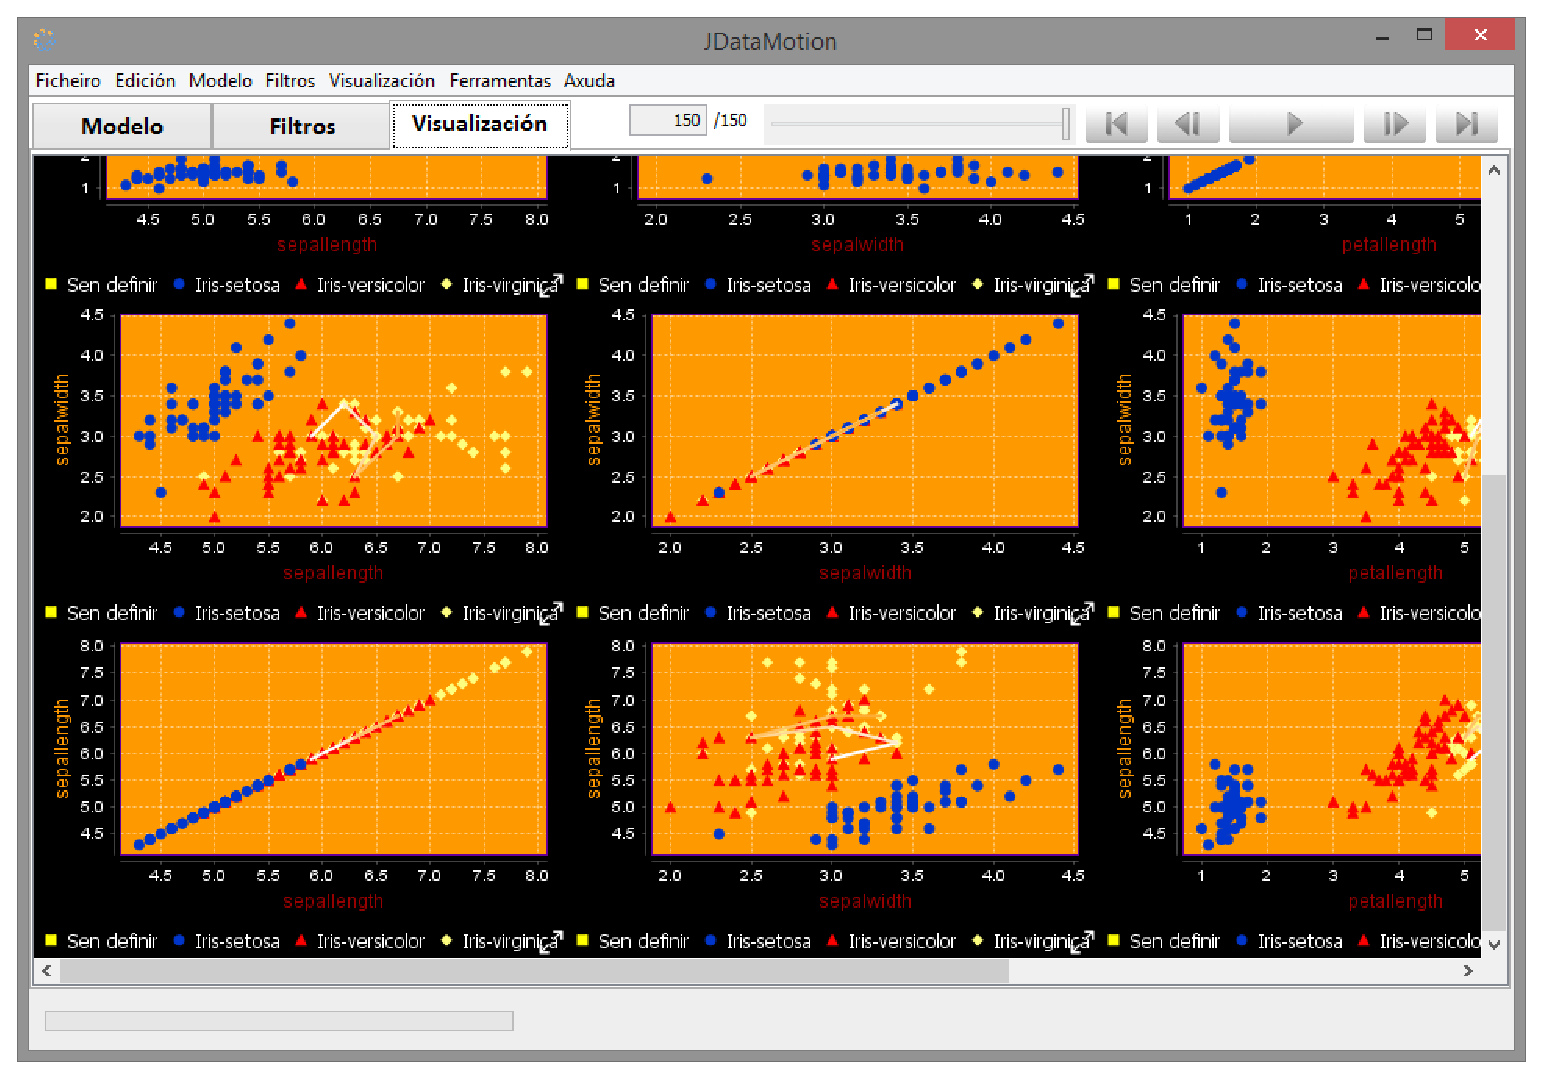
\includegraphics[width=\textwidth,height=\textheight,keepaspectratio]{figuras/RF11}
\caption{Comprobación heurística do RF11}
\label{RF11}
\end{figure}
\item[Resultado]
Correcto.
\end{description}

\subsubsection*{RF12}
\begin{description}
\item[Título] \hfill
Engadir diagramas de dispersión ao menú de visualización
\item[Descrición] \hfill
A aplicación debe permitir engadir dinamicamente novos diagramas de dispersión dentro do menú de visualización.
\item[Importancia] \hfill
Esencial
\item[Tipo de proba] \hfill
Avaliación heurística
\item[Descrición]
Abrimos un ficheiro ARFF ou CSV e imos á lapela de Visualización. Na barra de menús, iremos a Visualización \textgreater{} Engadir ou eliminar scatterplots e seleccionamos da matriz os elementos que queremos engadir á visualización.
\begin{figure}
\centering
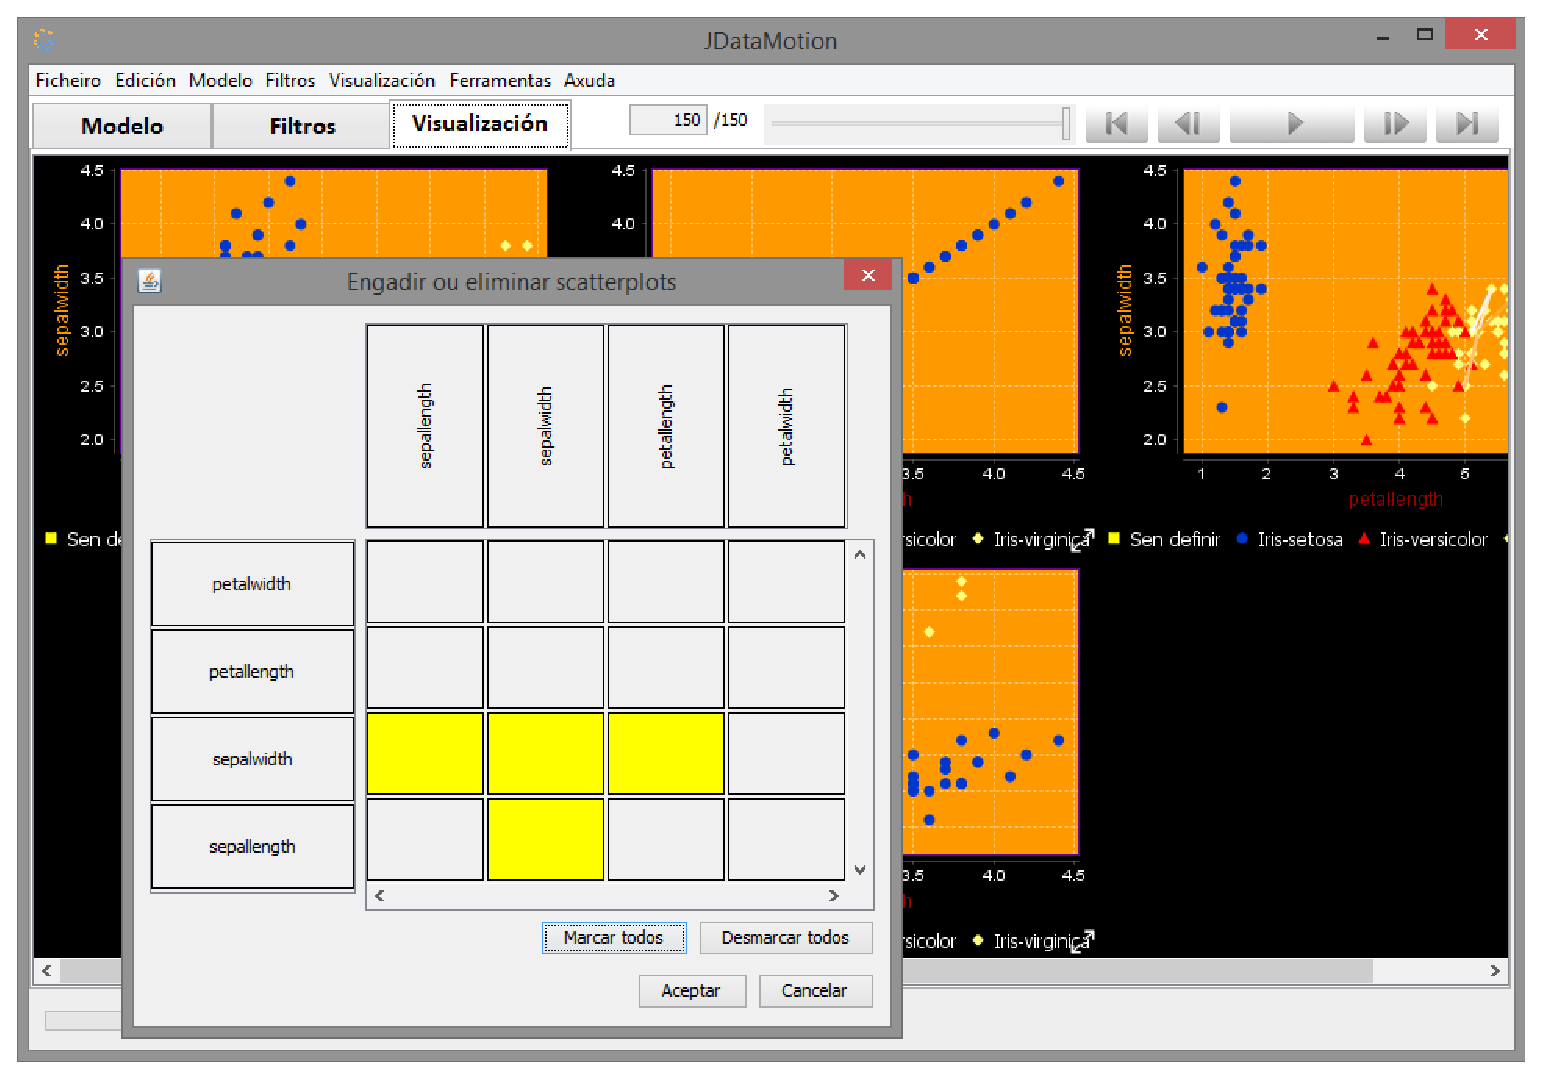
\includegraphics[width=\textwidth,height=\textheight,keepaspectratio]{figuras/RF1213}
\caption{Comprobación heurística do RF12}
\label{RF1213}
\end{figure}
\item[Resultado]
Correcto.
\end{description}

\subsubsection*{RF13}
\begin{description}
\item[Título] \hfill
Eliminar un diagrama de dispersión do menú de visualización
\item[Descrición] \hfill
A aplicación debe permitir eliminar un diagrama de dispersión do menú de visualización.
\item[Importancia] \hfill
Esencial
\item[Tipo de proba] \hfill
Avaliación heurística
\item[Descrición]
Consideramos que xa se esta visualizando algún scatterplot. Na barra de menús, iremos a Visualización \textgreater{} Engadir ou eliminar scatterplots e desmarcamos da matriz os elementos que queremos quitar da visualización.
\begin{figure}
\centering
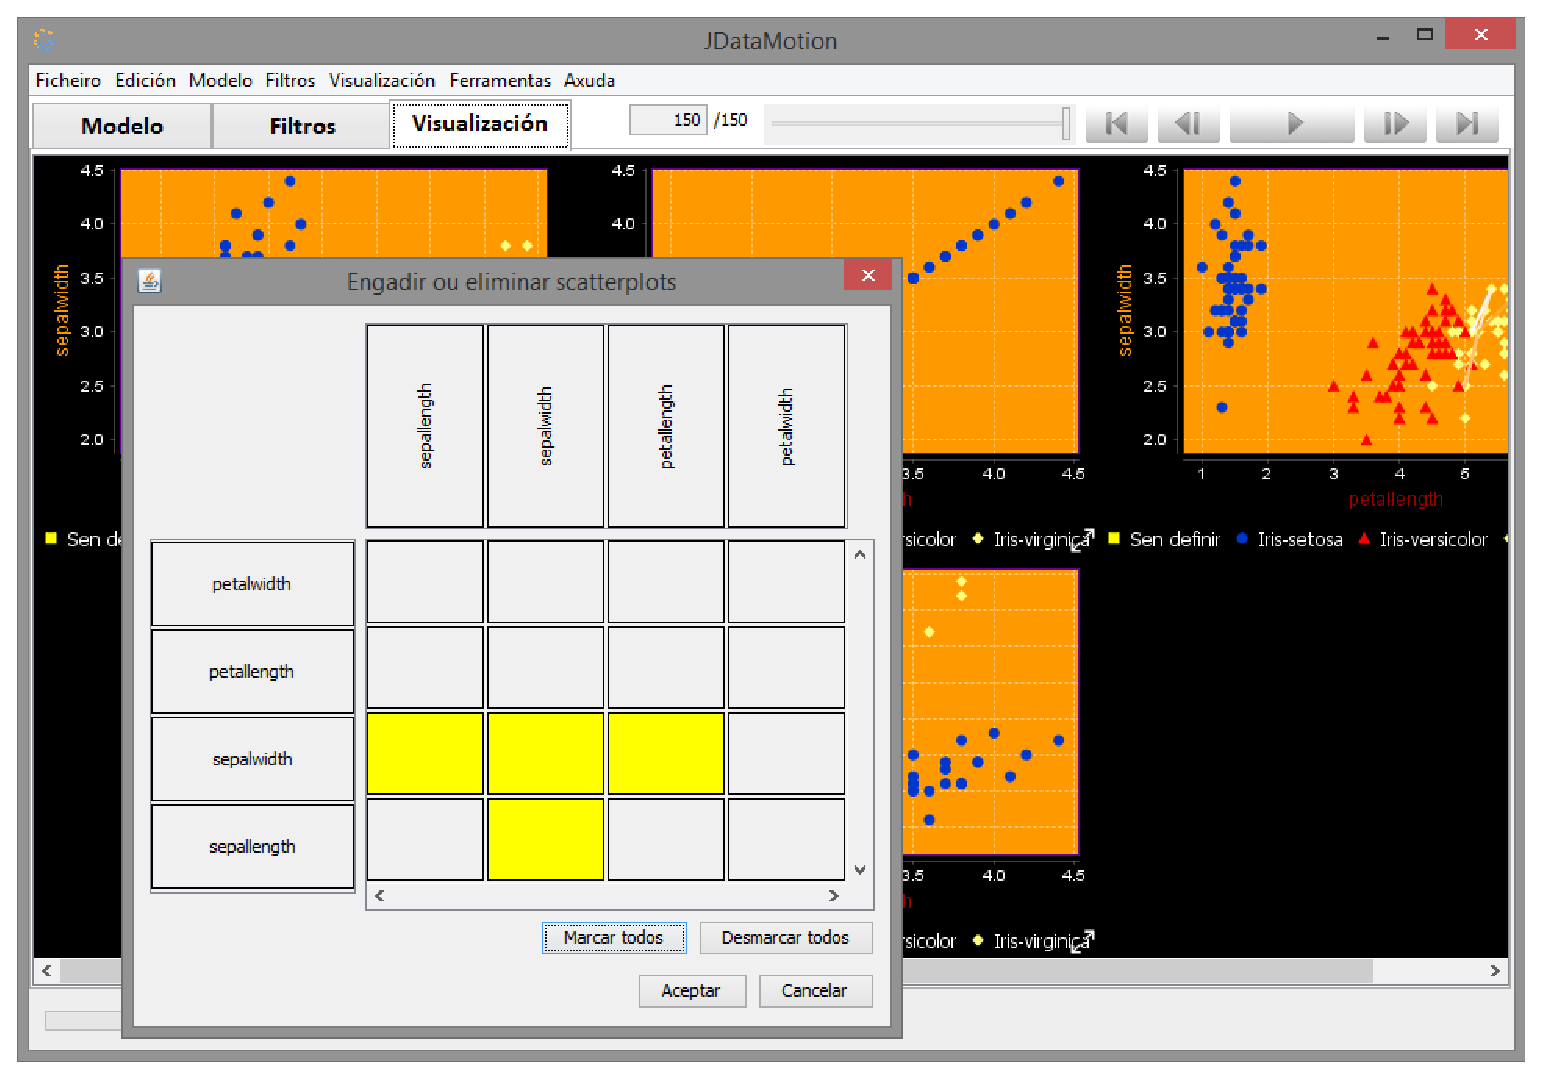
\includegraphics[width=\textwidth,height=\textheight,keepaspectratio]{figuras/RF1213}
\caption{Comprobación heurística do RF13}
\label{RF1213}
\end{figure}
\item[Resultado]
Correcto.
\end{description}

\subsubsection*{RF14}
\begin{description}
\item[Título] \hfill
Configurar diagramas de dispersión do menú de visualización
\item[Descrición] \hfill
A aplicación debe permitir especificar para os diagramas de dispersión do menú de visualización a súa configuración, respecto a que parámetros se representarán en cada un dos eixos ou si as cores e formas dos puntos se desexan usar para representar algún atributo nominal.
\item[Importancia] \hfill
Esencial
\item[Tipo de proba] \hfill
Avaliación heurística
\item[Descrición]
Para configurar os atributos representados en cada eixo está a matriz e3 selección de Visualización \textgreater{} Engadir ou eliminar scatterplots. (ver RF12 e RF13). Para representar un atributo de clase por medio de cores e formas diferentes, só temos que seleccionalo en Visualización \textgreater{} Establecer atributo nominal representado. Ao aceptar podemos apreciar o resultado.
\begin{figure}
\centering
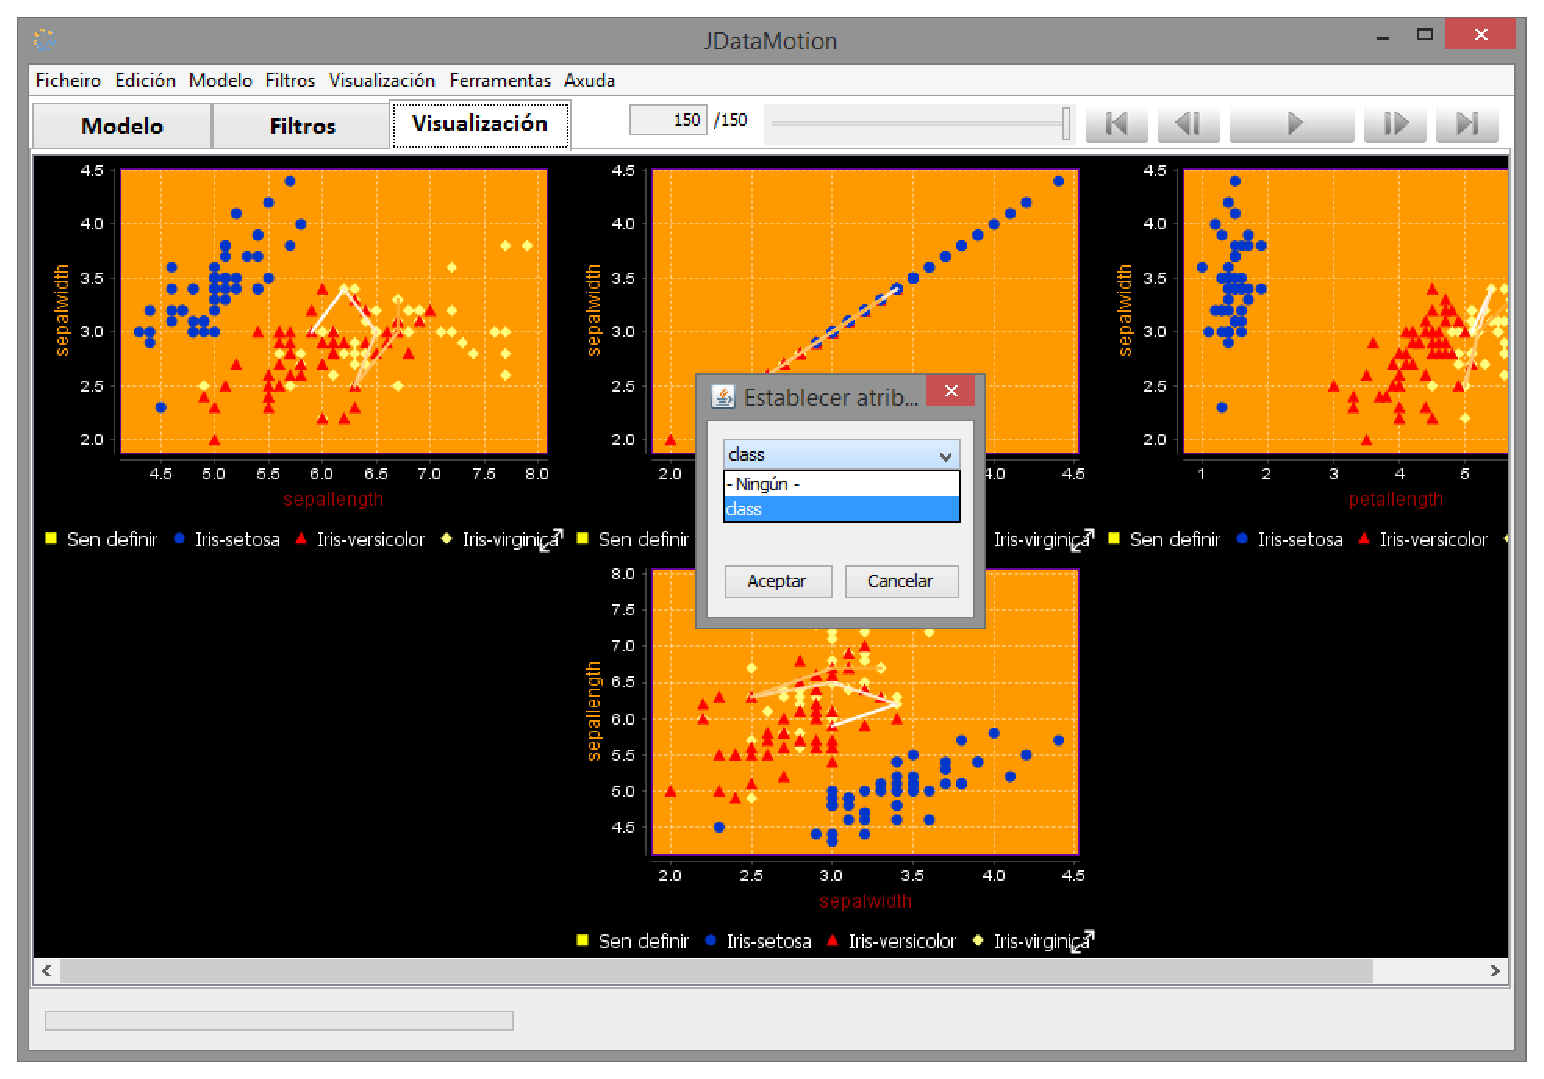
\includegraphics[width=\textwidth,height=\textheight,keepaspectratio]{figuras/RF14}
\caption{Comprobación heurística do RF14}
\label{RF14}
\end{figure}
\item[Resultado]
Correcto.
\end{description}

\subsubsection*{RF15}
\begin{description}
\item[Título] \hfill
Detallar punto seleccionado dentro do diagrama de dispersión
\item[Descrición] \hfill
Cada punto dos diagramas de dispersión pode ser seleccionado para ver nun apartado os seus detalles (todos os seus atributos).
\item[Importancia] \hfill
Esencial
\item[Tipo de proba] \hfill
Avaliación heurística
\item[Descrición]
Tendo algún diagrama representado podemos apreciar este efecto pulsando preto de calquera punto. Abrirase un menú que detalle o punto seleccionado, ou unha lista deles (puntos solapados).
\begin{figure}
\centering
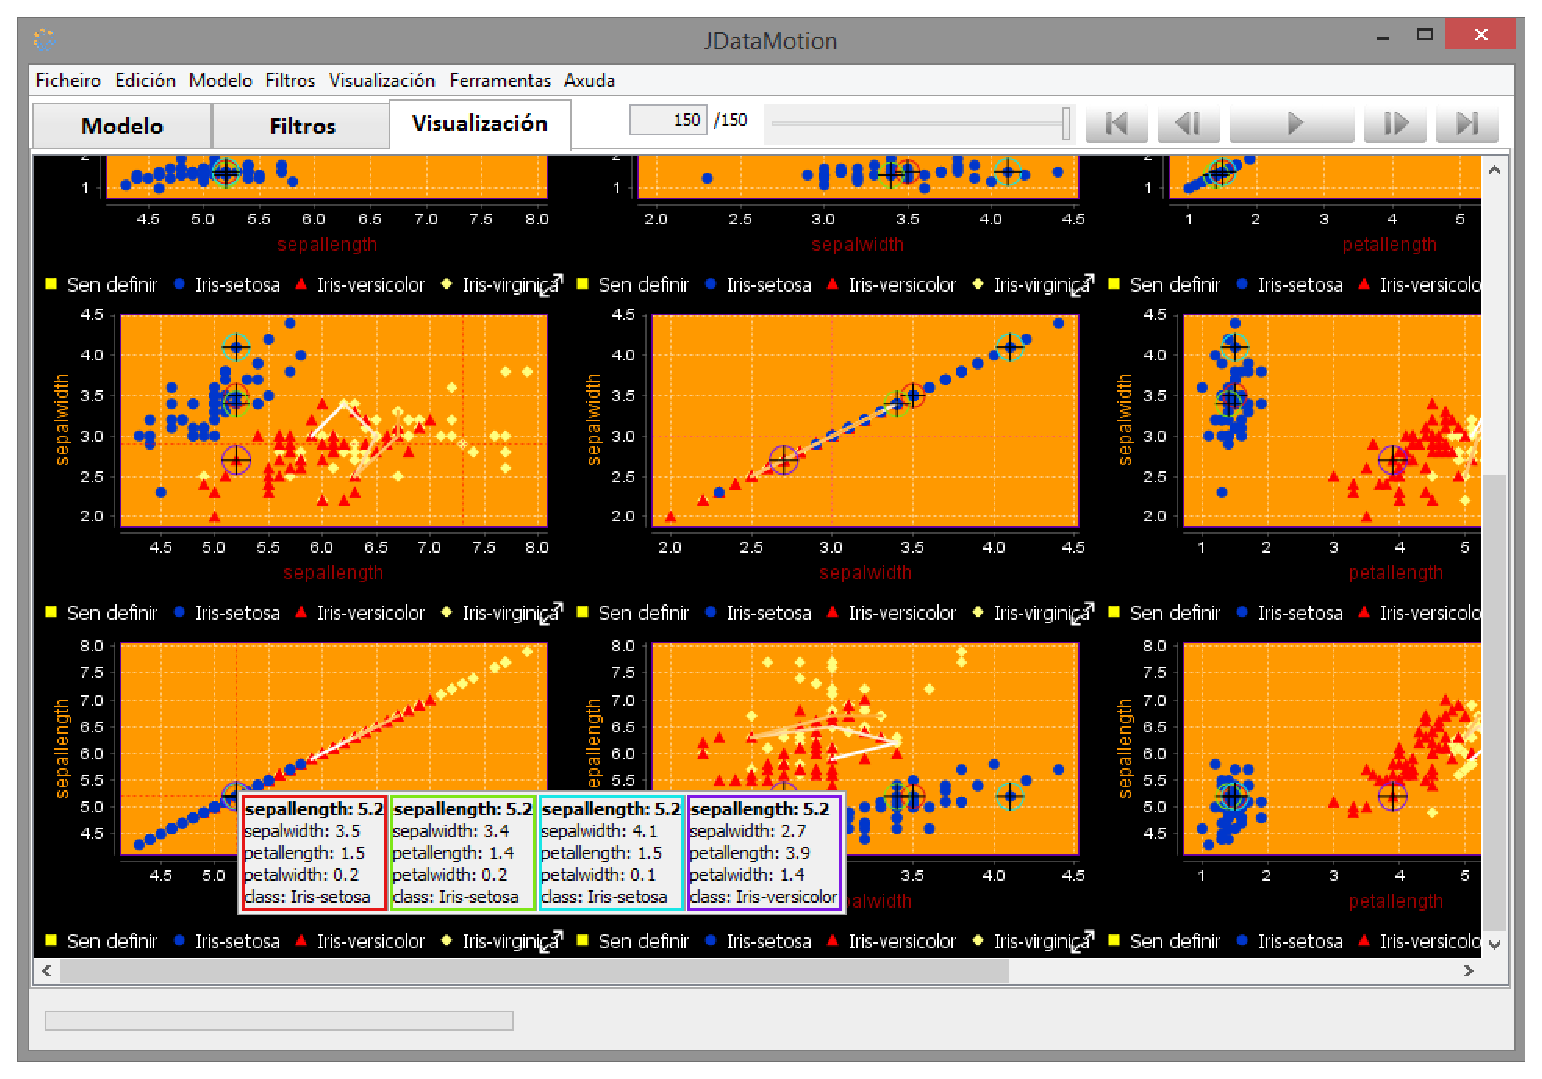
\includegraphics[width=\textwidth,height=\textheight,keepaspectratio]{figuras/RF1516}
\caption{Comprobación heurística do RF15}
\label{RF1516}
\end{figure}
\item[Resultado]
Correcto.
\end{description}

\subsubsection*{RF16}
\begin{description}
\item[Título] \hfill
Resaltar punto en diagramas de dispersión
\item[Descrición] \hfill
Cada punto seleccionalo dentro dun diagrama de dispersión resaltarase tanto nel coma en todos os demais diagramas de dispersión (que plasmarán outras proxeccións do mesmo punto).
\item[Importancia] \hfill
Esencial
\item[Tipo de proba] \hfill
Avaliación heurística
\item[Descrición]
Tendo algúns diagramas representados podemos apreciar este efecto pulsando nun punto no que haxa algún outro punto coincidindo nesa mesma posición (puntos solapados). As proyeccións desos puntos noutros diagramas tamén se resaltan, mantendo o mesmo color as que referencian a mesma instancia.
\begin{figure}
\centering
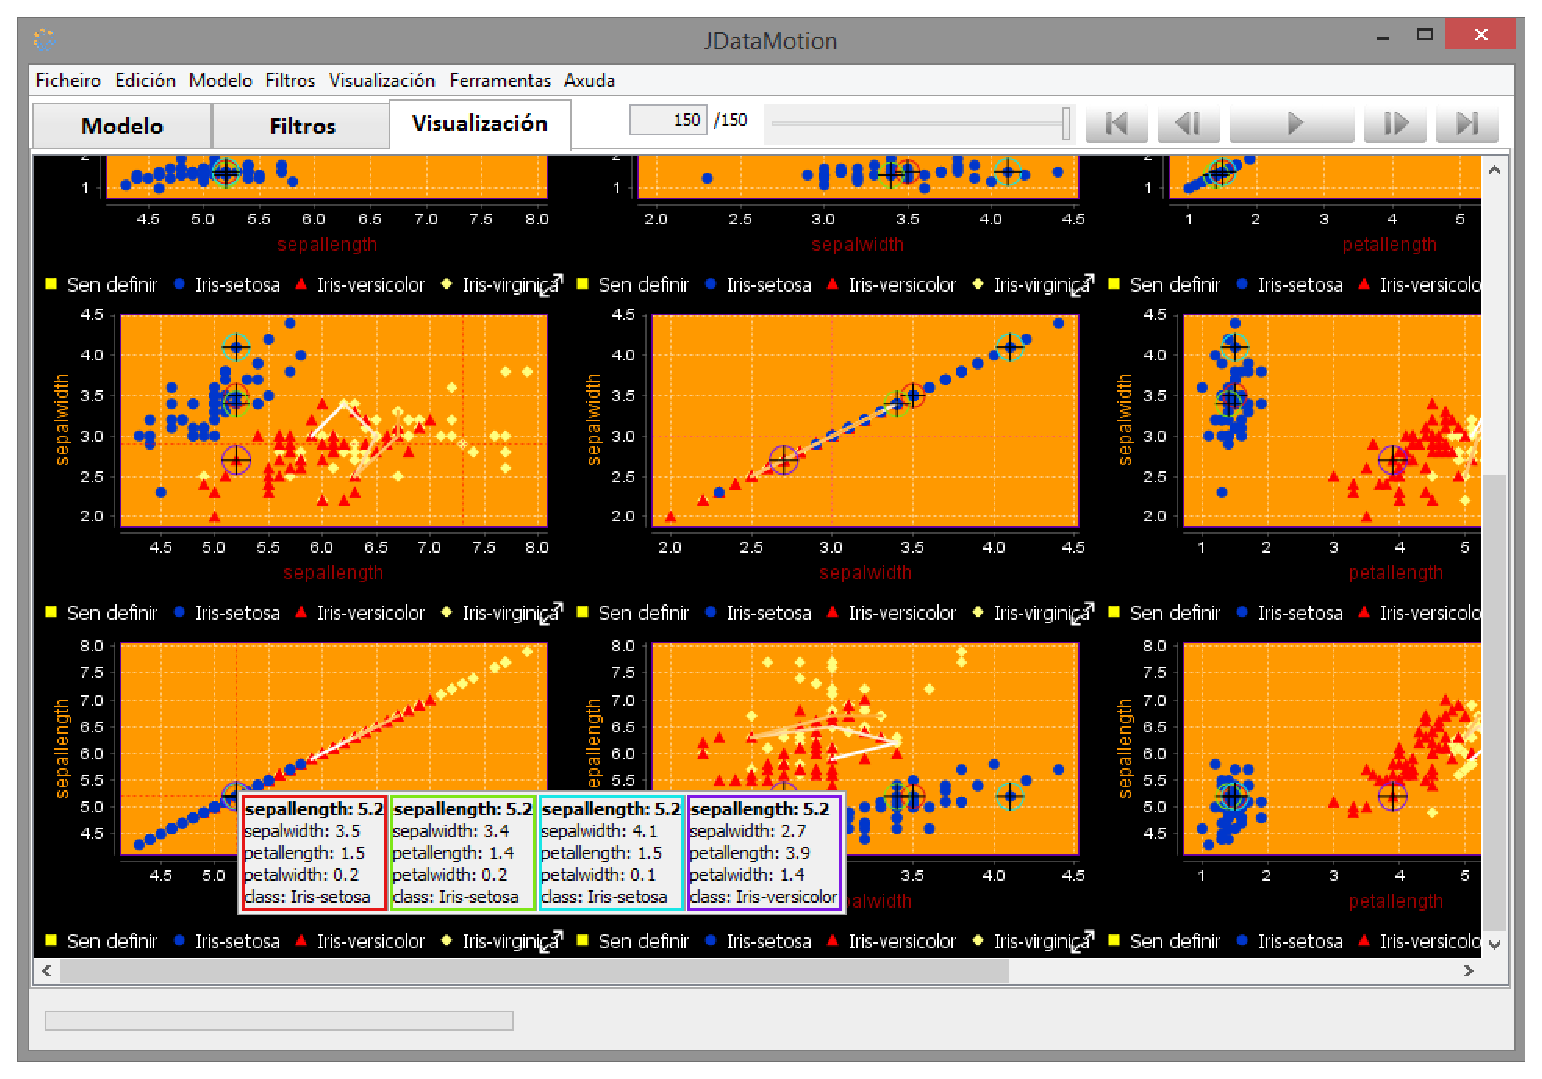
\includegraphics[width=\textwidth,height=\textheight,keepaspectratio]{figuras/RF1516}
\caption{Comprobación heurística do RF16}
\label{RF1516}
\end{figure}
\item[Resultado]
Correcto.
\end{description}

\subsubsection*{RF17}
\begin{description}
\item[Título] \hfill
Desprazar a ventá de visualización por arrastre de cada diagrama de dispersión
\item[Descrición] \hfill
Para cada diagrama de dispersión poderemos usar unha ferramenta ``man'' para desprazar a ventá polo diagrama de dispersión.
\item[Importancia] \hfill
Esencial
\item[Tipo de proba] \hfill
Avaliación heurística
\item[Descrición]
Tendo algún diagrama representado podemos apreciar este efecto pulsando a tecla Control e arrastrando co rato un diagrama de dispersión. Veremos como a ventá que enfoca o gráfico se despraza na dirección que marquemos.
\begin{figure}
\centering
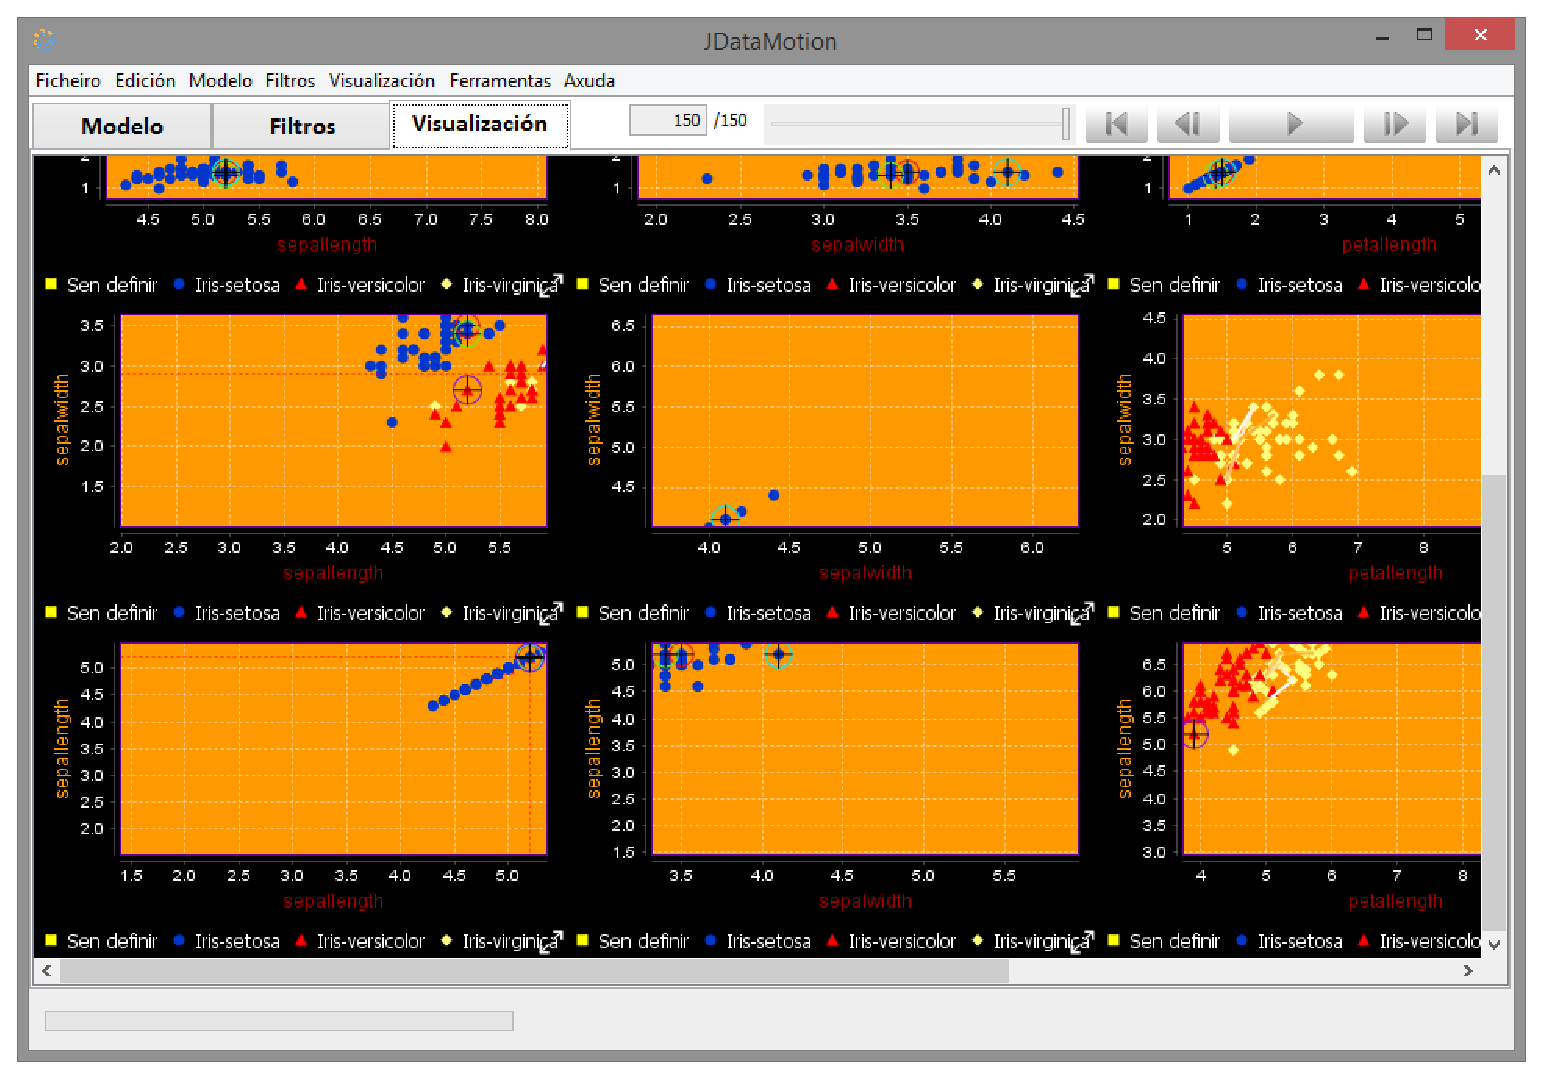
\includegraphics[width=\textwidth,height=\textheight,keepaspectratio]{figuras/RF17}
\caption{Comprobación heurística do RF17}
\label{RF17}
\end{figure}
\item[Resultado]
Correcto.
\end{description}

\subsubsection*{RF18}
\begin{description}
\item[Título] \hfill
Escalar a ventá de visualización de cada diagrama de dispersión
\item[Descrición] \hfill
Para cada diagrama de dispersión poderemos usar unha ferramenta de escalado da ventá para facer zoom no diagrama de dispersión.
\item[Importancia] \hfill
Esencial
\item[Tipo de proba] \hfill
Avaliación heurística
\item[Descrición]
Tendo algún diagrama representado podemos apreciar este efecto colocando o cursor enriba dun diagrama e xirando a roda do rato. Veremos como a ventá de visualización do diagrama escala. Tamén se pode probar pulsando co botón secundario nun diagrama e seleccionando unha opción dentro de Acercar ou Alonxar.
\begin{figure}
\centering
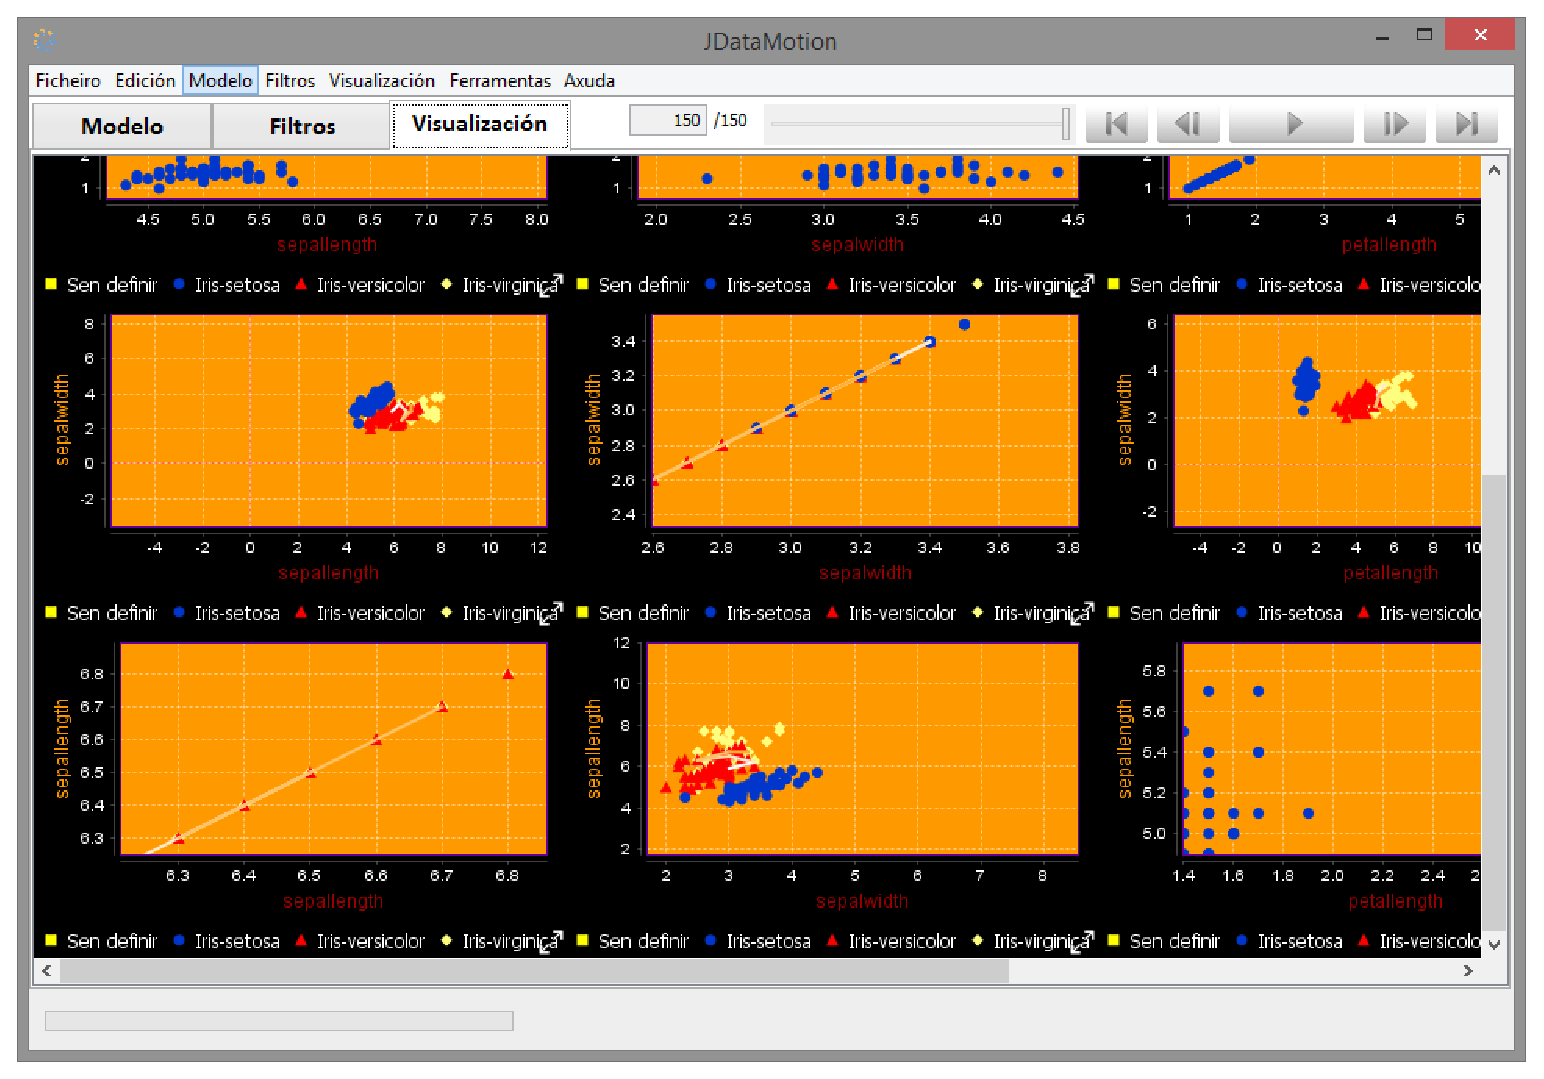
\includegraphics[width=\textwidth,height=\textheight,keepaspectratio]{figuras/RF18}
\caption{Comprobación heurística do RF18}
\label{RF18}
\end{figure}
\item[Resultado]
Correcto.
\end{description}

\subsubsection*{RF19}
\begin{description}
\item[Título] \hfill
Escalar e reposicionar dinamicamente
\item[Descrición] \hfill
Para cada diagrama de dispersión permitirase que a ventá de visualización que o enfoca se adapte dinamicamente ao conxunto de datos representados (movéndose, afastándose e aproximándose para englobar todos os datos).
\item[Importancia] \hfill
Esencial
\item[Tipo de proba] \hfill
Avaliación heurística
\item[Descrición]
Tendo algún diagrama representado podemos apreciar este efecto colocando o cursor enriba dun diagrama e xirando a roda do rato. Veremos como a ventá de visualización do diagrama escala.
\begin{figure}
\centering
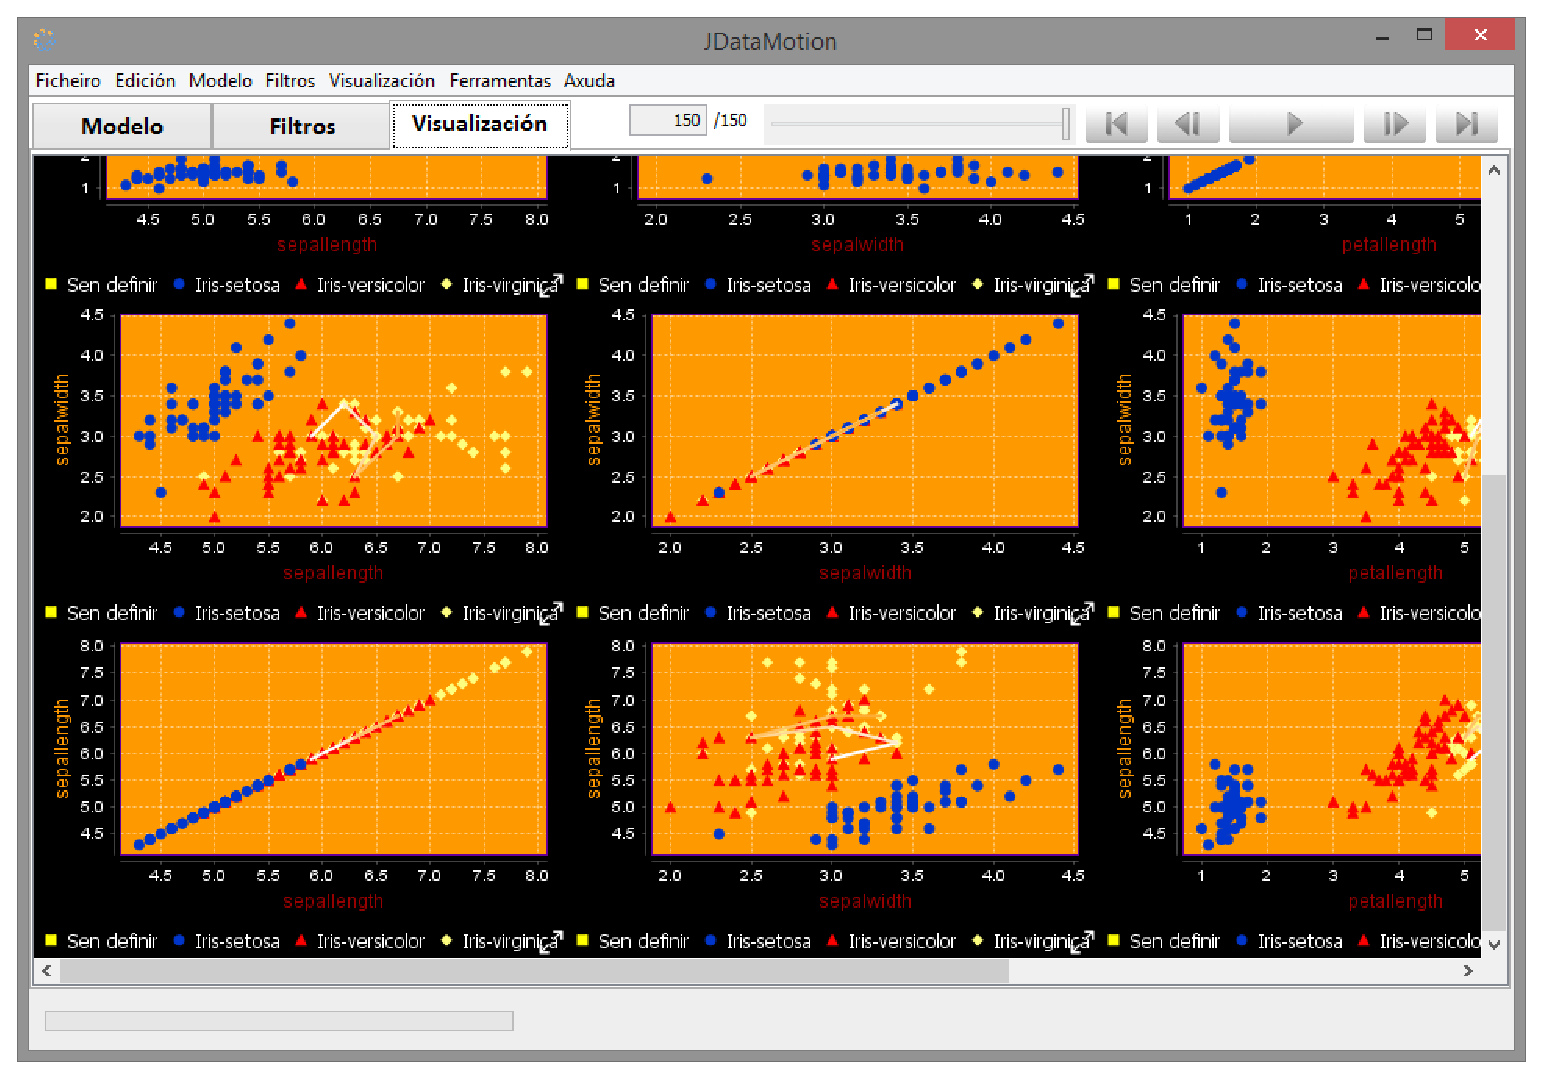
\includegraphics[width=\textwidth,height=\textheight,keepaspectratio]{figuras/RF19}
\caption{Comprobación heurística do RF19}
\label{RF19}
\end{figure}
\item[Resultado]
Correcto.
\end{description}

\subsubsection*{RF20}
\begin{description}
\item[Título] \hfill
Reproducir a secuencia de datos
\item[Descrición] \hfill
A aplicación debe de permitir que a visualización dos diagramas de dispersión poida basearse na variable temporal (ou de orde) para reproducir a secuencia de datos, amosando os datos de cada diagrama de dispersión baixo unha secuencia de vídeo. Nesta secuencia engadiríase á visualización en cada instante a tupla de atributos asociada a esa marca temporal. 
\item[Importancia] \hfill
Esencial
\item[Tipo de proba] \hfill
Avaliación heurística
\item[Descrición]
Tendo algún diagrama representado, volvemos ao Modelo e seleccionamos un atributo numérico ou String (pero cun formato de tempo) pinchando nel co botón secundario. Marcámolo como índice temporal. Agora imos a Visualización \textgreater{} Configurar reprodución e personalizamos os valores que se amosan. Para que se teña en conta o índice temporal, seleccionaremos en Orde do modelo a opción ``Orde dos índices temporais numéricos'' ou ben ``Orde dos índices temporais numéricos ponderados'', en función de si o índice temporal expresa só orde ou unha duración relativa, respectivamente. Con todo isto, ao premer no botón de reprodución do menú Visualización comezaremos a ver a secuencia de puntos avanzar da forma que acabamos de configurar.
\begin{figure}
\centering
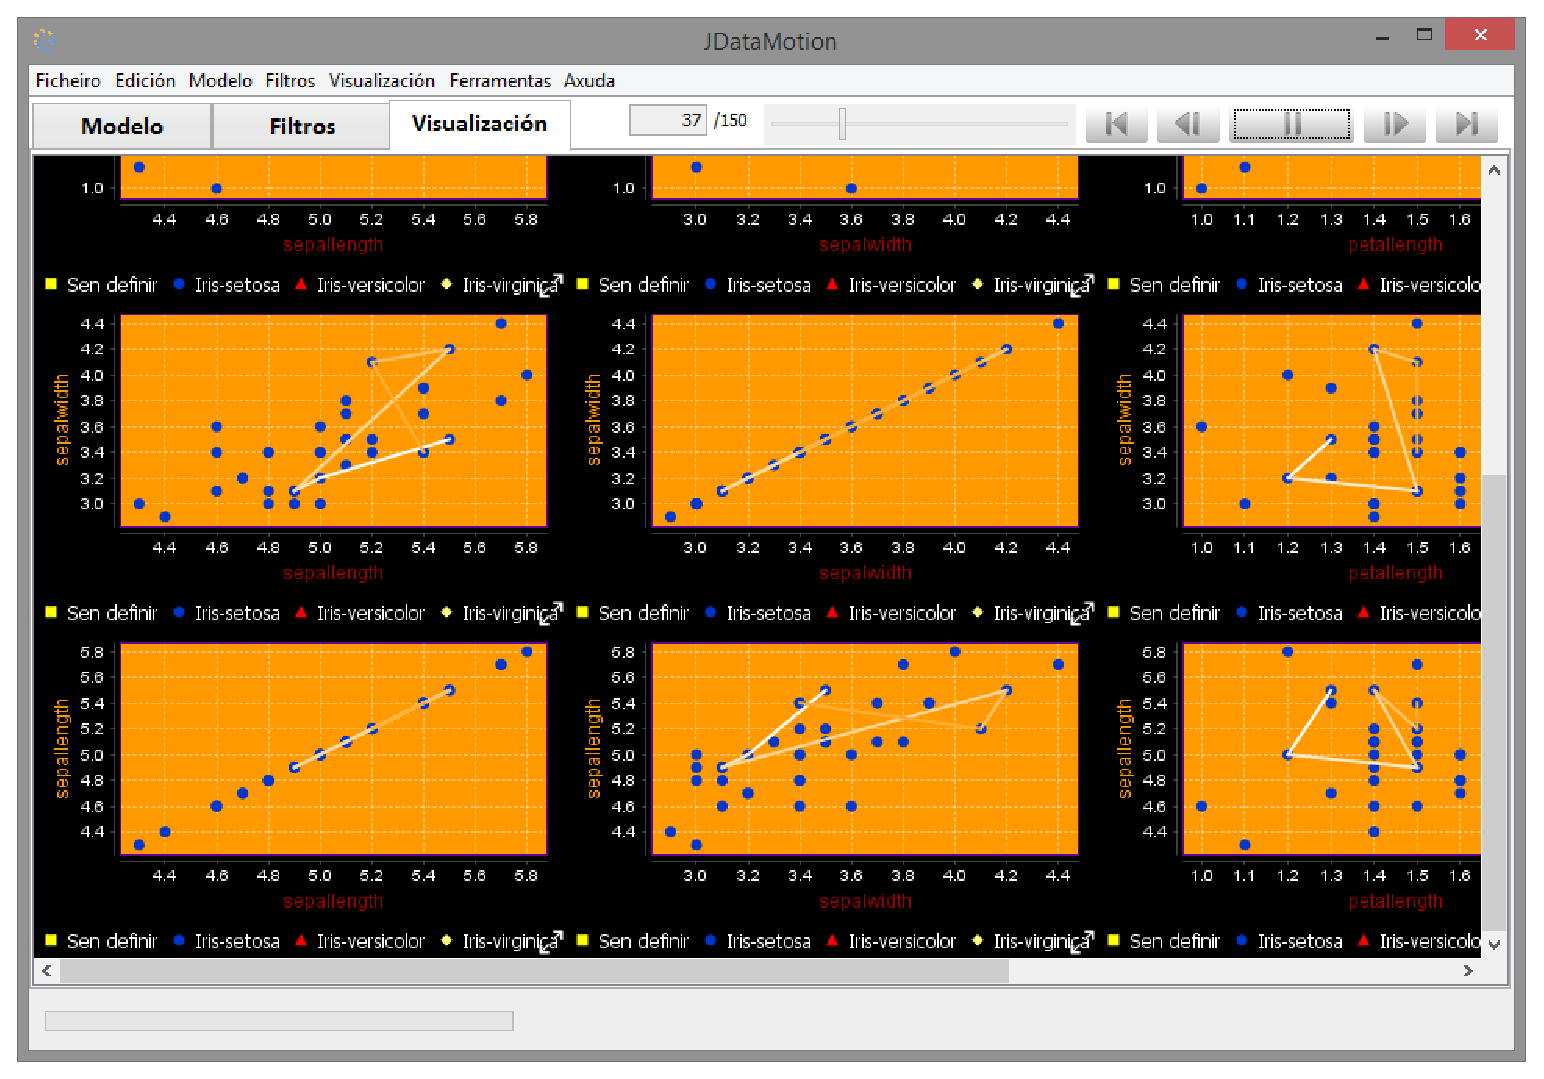
\includegraphics[width=\textwidth,height=\textheight,keepaspectratio]{figuras/RF202122}
\caption{Comprobación heurística do RF20}
\label{RF202122}
\end{figure}
\item[Resultado]
Correcto.
\end{description}

\subsubsection*{RF21}
\begin{description}
\item[Título] \hfill
Representar estela
\item[Descrición] \hfill
A aplicación debe de permitir que cada novo punto pintado se ligue ao último representado no diagrama de dispersión por medio dunha liña recta.
\item[Importancia] \hfill
Esencial
\item[Tipo de proba] \hfill
Avaliación heurística
\item[Descrición]
Tendo algún diagrama representado, imos a Visualización \textgreater{} Configurar reprodución e asegurámonos de que o valor da lonxitude de estela non sexa 0. Entón premendo no botón de reproducir veremos que a estela abarcará o número de puntos especificado, tendo a súa cabeza no último punto que se visualiza en cada momento.
\begin{figure}
\centering
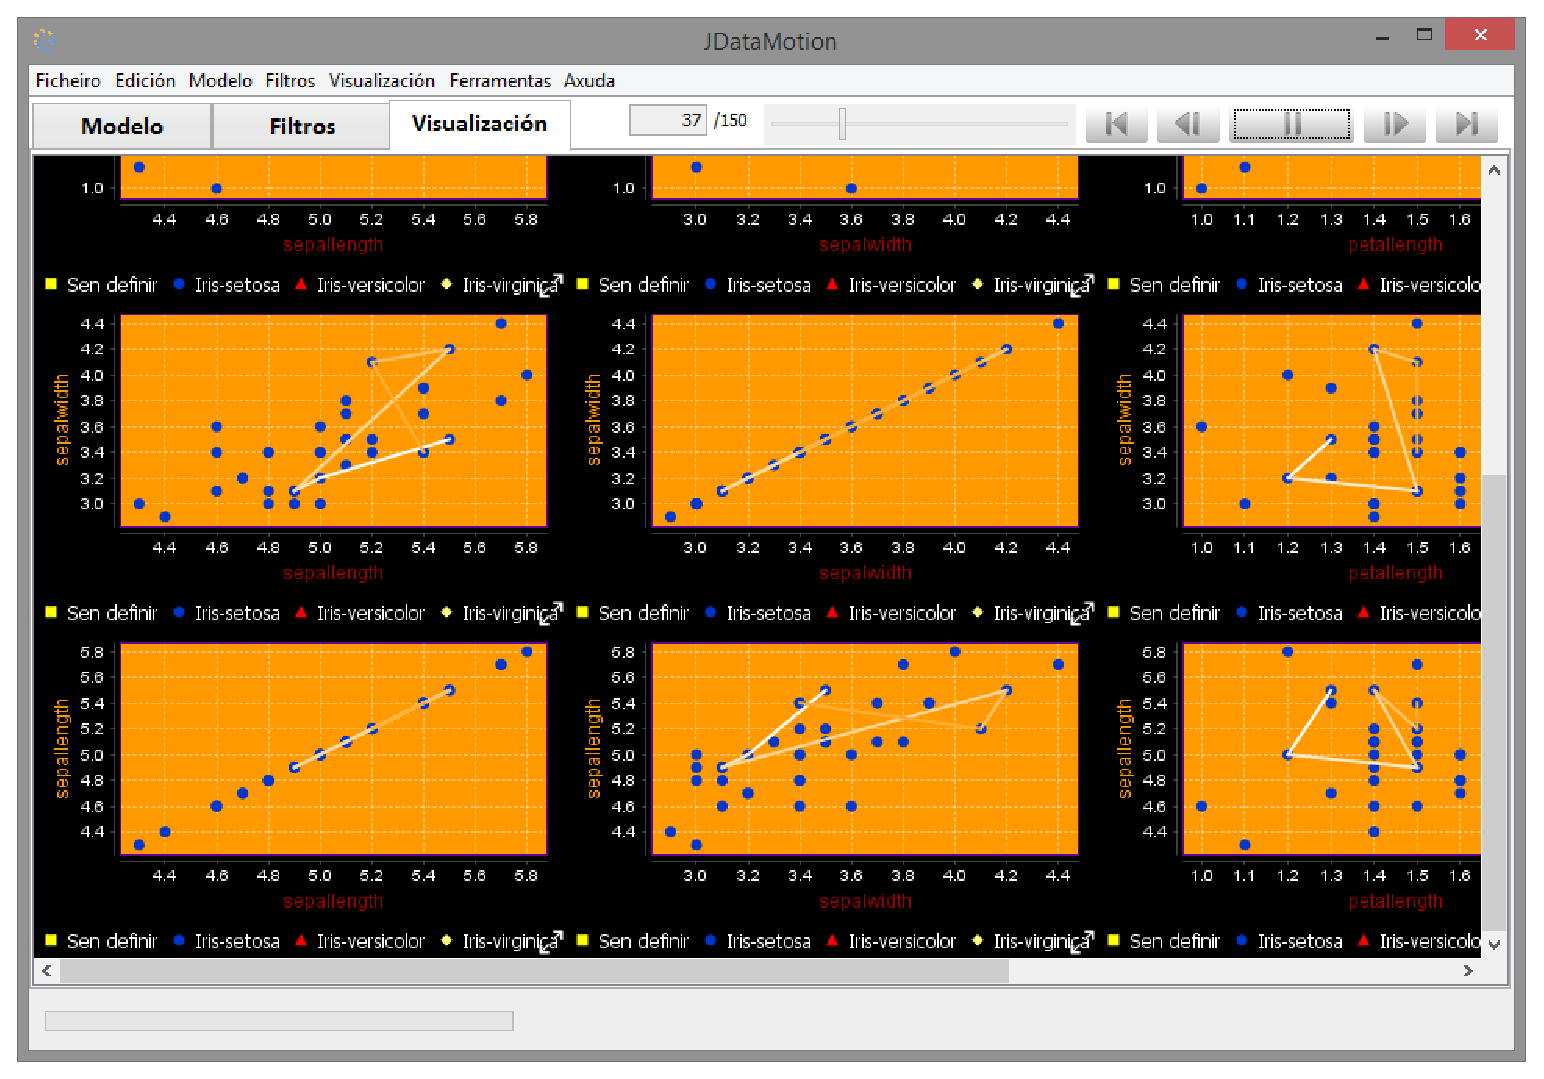
\includegraphics[width=\textwidth,height=\textheight,keepaspectratio]{figuras/RF202122}
\caption{Comprobación heurística do RF21}
\label{RF202122}
\end{figure}
\item[Resultado]
Correcto.
\end{description}

\subsubsection*{RF22}
\begin{description}
\item[Título] \hfill
Difuminar estela ao longo da reprodución
\item[Descrición] \hfill
A aplicación debe permitir difuminar as estelas xa representadas a través do avance temporal.
\item[Importancia] \hfill
Esencial
\item[Tipo de proba] \hfill
Avaliación heurística
\item[Descrición]
Tendo algún diagrama representado, imos a Visualización \textgreater{} Configurar reprodución e asegurámonos de que o valor da lonxitude de estela sexa un número significativo. Entón premendo no botón de reproducir veremos que a estela abarcará o número de puntos especificado, tendo unha cor máis intensa nos tramos nos que une puntos máis recentes, e máis tenue naqueles con maior antigüidade.
\begin{figure}
\centering
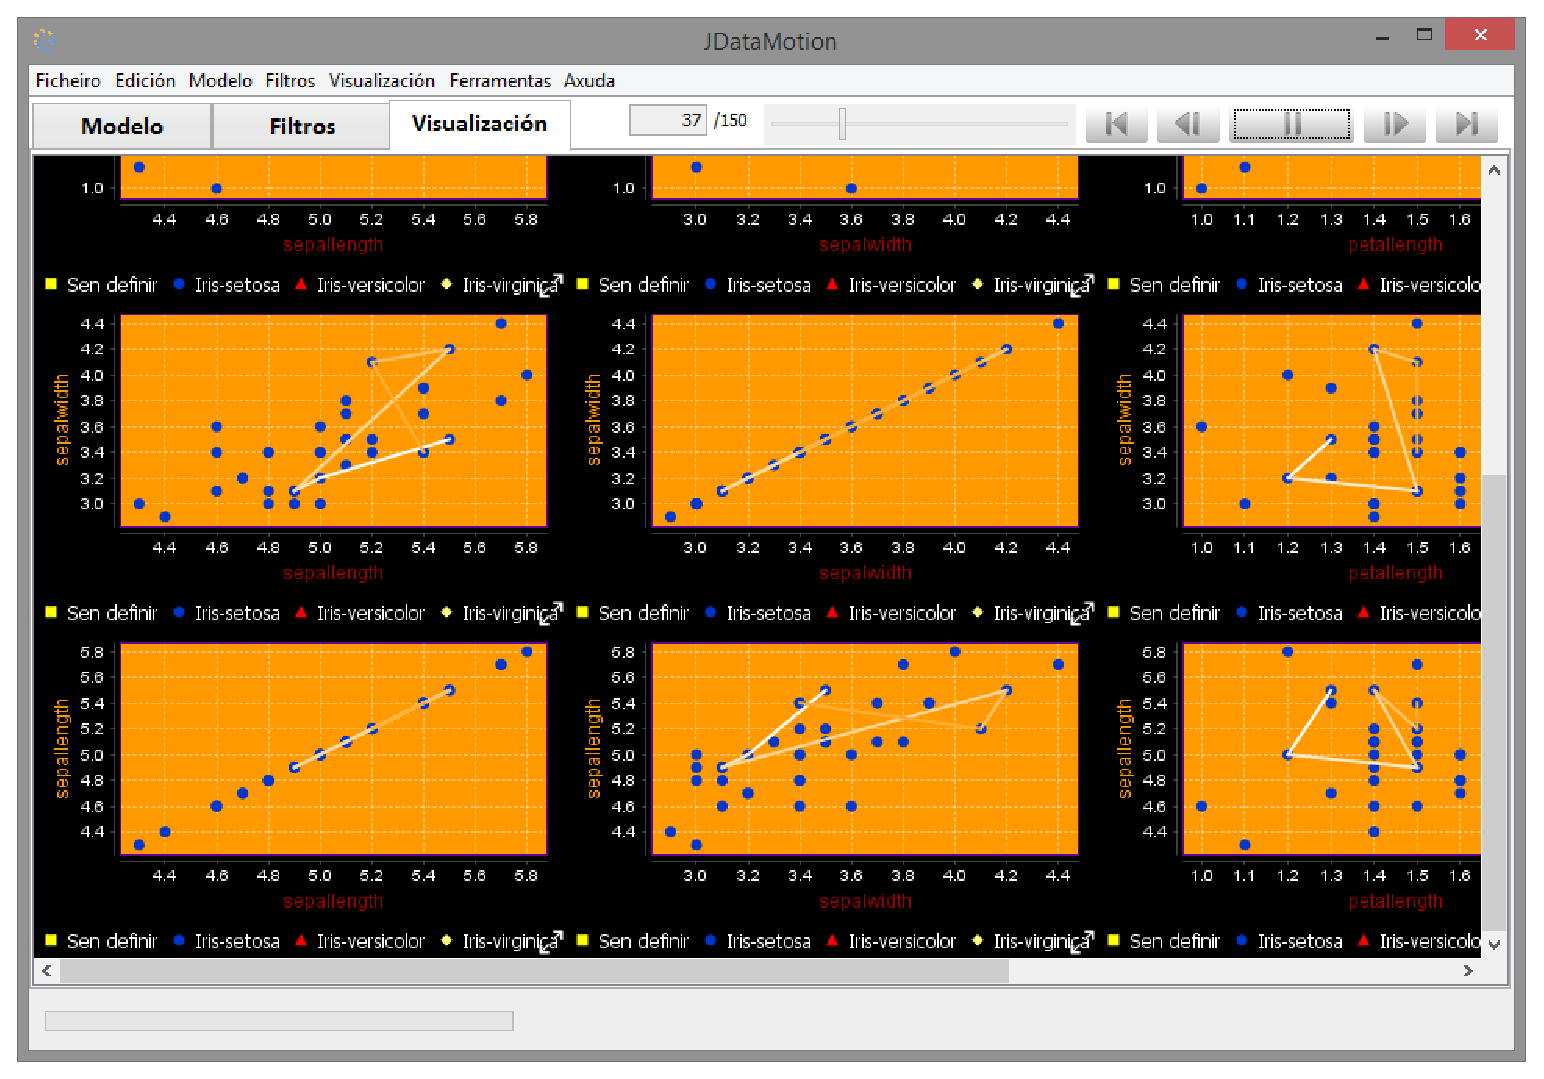
\includegraphics[width=\textwidth,height=\textheight,keepaspectratio]{figuras/RF202122}
\caption{Comprobación heurística do RF22}
\label{RF202122}
\end{figure}
\item[Resultado]
Correcto.
\end{description}

\subsubsection*{RF23}
\begin{description}
\item[Título] \hfill
Configurar a reprodución da secuencia de datos
\item[Descrición] \hfill
A aplicación debe de permitir que a visualización dos diagramas de dispersión sexa configurable en canto a tempo transcorrido entre marcas temporais. Para a reprodución usando marcas temporais ponderadas, este tempo representará a separación entre as dúas marcas temporais mais próximas (tempo mínimo). Ademáis débese poder especificar o número de marcas temporais que durará o difuminado dos puntos que se ploteen, de xeito que durante ese intervalo cada punto se vaia difuminando ata desaparecer. Pode ser igual a 0 para que os puntos non se difuminen.
\item[Importancia] \hfill
Esencial
\item[Tipo de proba] \hfill
Avaliación heurística
\item[Descrición]
Tendo algún diagrama representado, volvemos ao Modelo e seleccionamos un atributo numérico ou String (pero cun formato de tempo) pinchando nel co botón secundario. Marcámolo como índice temporal. Agora imos a Visualización \textgreater{}. Para que se teña en conta o índice temporal, seleccionaremos en Orde do modelo a opción ``Orde dos índices temporais numéricos ponderados''. Con todo isto, ao premer no botón de reprodución do menú Visualización comezaremos a ver a secuencia de puntos avanzar da forma que acabamos de configurar. O difuminado dos puntos non se pode probar porque non foi implementado todavía (debido a unha restricción das estruturas do Dataset que non permitían a reprodución cara atrás).
\begin{figure}
\centering
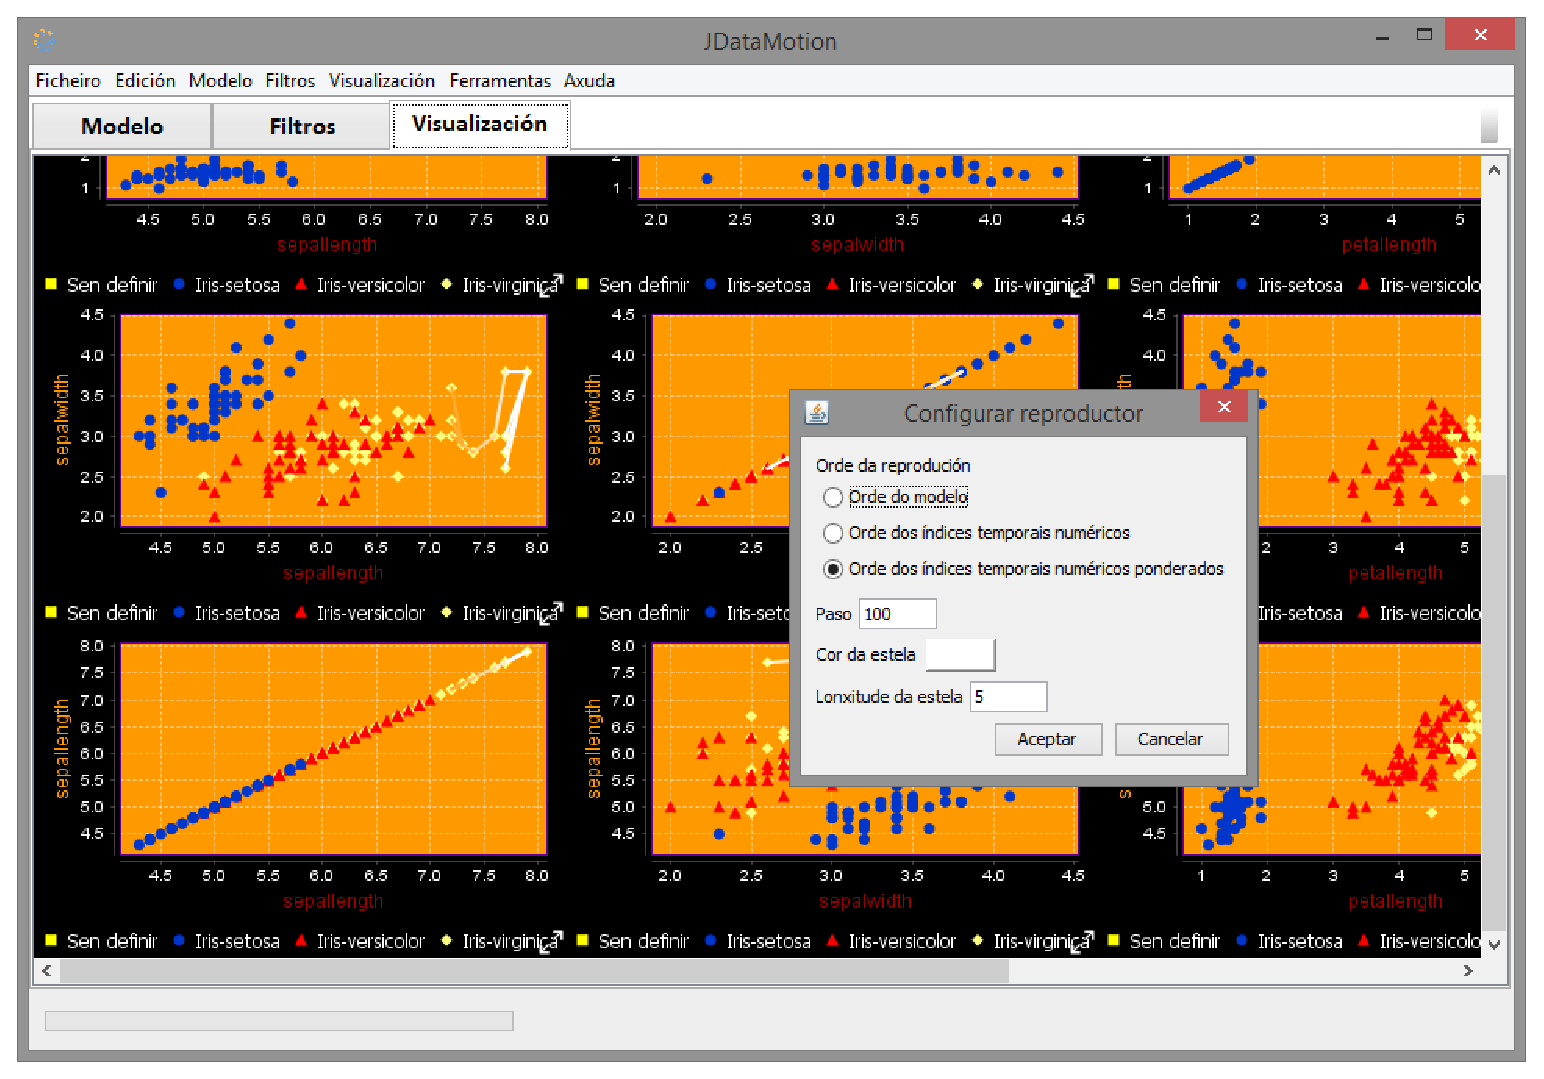
\includegraphics[width=\textwidth,height=\textheight,keepaspectratio]{figuras/RF23}
\caption{Comprobación heurística do RF23}
\label{RF23}
\end{figure}
\item[Resultado]
Correcto.
\end{description}

\subsubsection*{RF24}
\begin{description}
\item[Título] \hfill
Pausar a reprodución
\item[Descrición] \hfill
A aplicación debe permitir parar a reprodución na marca de tempo na que se atope ao executar esta acción, mantendo as visualizacións para ese momento.
\item[Importancia] \hfill
Esencial
\item[Tipo de proba] \hfill
Avaliación heurística
\item[Descrición]
Tendo algún diagrama representado e coa reprodución en curso, prememos outra vez no botón de reprodción (que agora terá un símbolo de dúas barras verticais paralelas). Comprobamos que todos os diagramas deteron a súa reprodución.
\begin{figure}
\centering
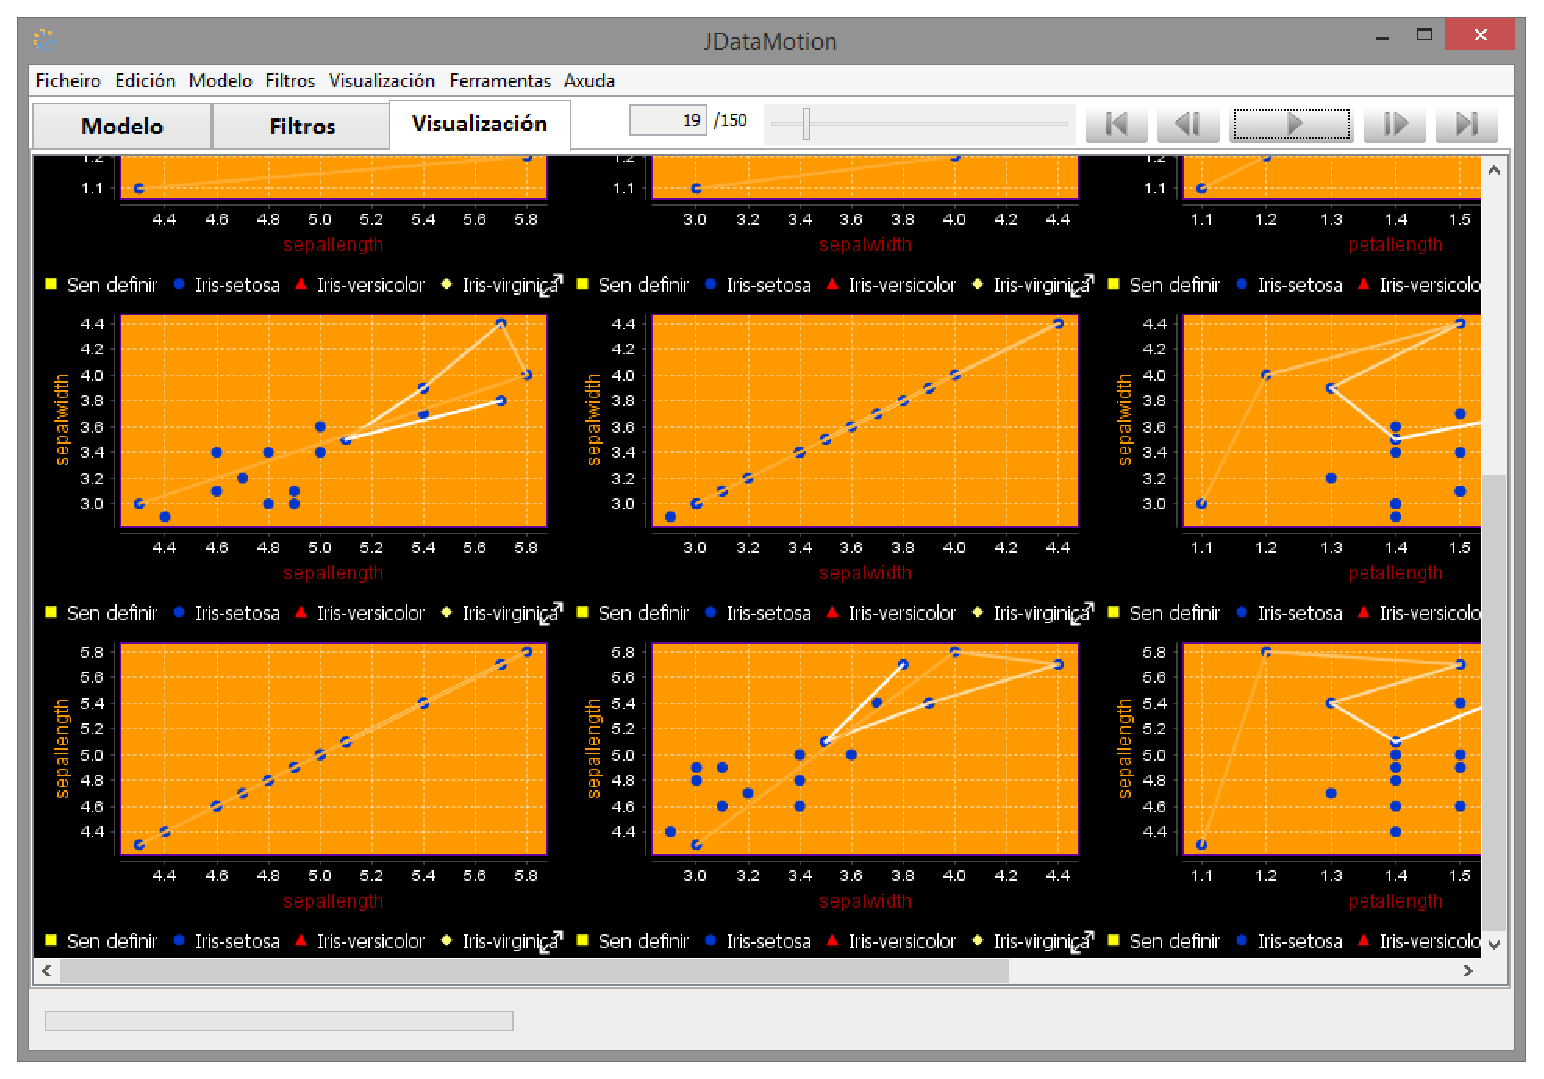
\includegraphics[width=\textwidth,height=\textheight,keepaspectratio]{figuras/RF24}
\caption{Comprobación heurística do RF24}
\label{RF24}
\end{figure}
\item[Resultado]
Correcto.
\end{description}

\subsubsection*{RF25}
\begin{description}
\item[Título] \hfill
Ir a un determinado instante dentro do intervalo temporal da reprodución
\item[Descrición] \hfill
A aplicación debe permitir situarse directamente sobre un instante de tempo, mantendo a reprodución pausada sobre esa marca temporal, e visualizando os diagramas de dispersión tal e como deben estar nese momento.
\item[Importancia] \hfill
Esencial
\item[Tipo de proba] \hfill
Avaliación heurística
\item[Descrición]
Tendo algún diagrama representado, observamos o desprazador que está no menú de Visualización, ao lado dos demais botóns de reprodución. Arrastramos o seu pivote por todo o ancho e observamos como aparecen (cando nos movemos acara a dereita) ou se agochan (cando nos movemos cara a esquerda) puntos en todos os diagramas. Soltando o pivote nunha posición a reprodución establécese nela, seguindo a partir de aí no caso de reanudarse.
\begin{figure}
\centering
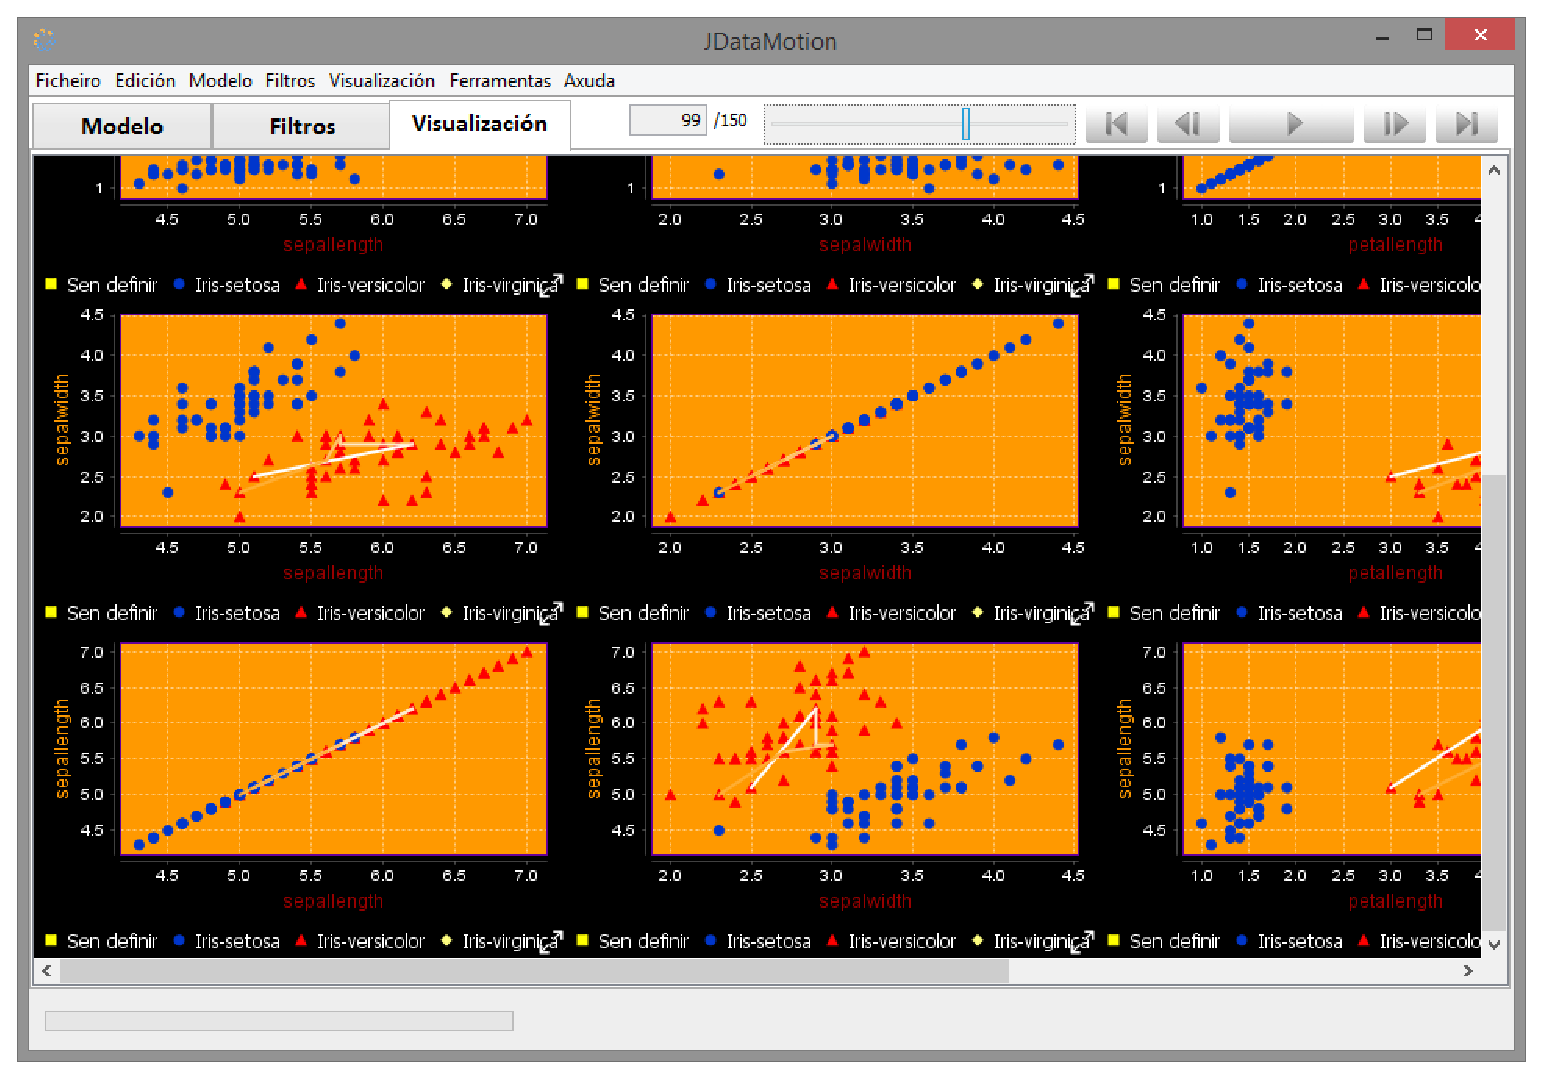
\includegraphics[width=\textwidth,height=\textheight,keepaspectratio]{figuras/RF25}
\caption{Comprobación heurística do RF25}
\label{RF25}
\end{figure}
\item[Resultado]
Correcto.
\end{description}

\subsubsection*{RF26}
\begin{description}
\item[Título] \hfill
Insertar filtros para os datos do experimento
\item[Descrición] \hfill
A aplicación debe permitir engadir unha serie de filtros que se aplicarán de xeito secuencial sobre a secuencia de datos coa que se esté a traballar. Chamarémoslle ``secuencia de filtros'' a esta secuencia.
\item[Importancia] \hfill
Esencial
\item[Tipo de proba] \hfill
Test implementado en JUnit.
\item[Nome do test] \hfill
TestRF2628
\item[Código fonte]
\begin{lstlisting}
    public void test() {
        Modelo modelo = new Modelo();
        Vista vista = new Vista();
        vista.inicializar(modelo, false);
        Controlador.setDebug(true);
        String resource = "example01.arff";
        IFilter filtro = new FiltroLimite();
        Double maximo = 15.0;
        int columna = 1;
        StringParameter sp1 = new StringParameter(), sp2 = new StringParameter();
        DoubleParameter sp3 = new DoubleParameter();
        sp1.setValue(recursosIdioma.getString("limiteValor"));
        sp2.setValue(recursosIdioma.getString("cotaSuperior"));
        sp3.setValue(maximo);
        try {
            String pathEntrada = new URI(getClass().getResource(resource).toString()).getPath();
            ComparableInstances is1 = ValidFileLoading.loadARFF(pathEntrada);
            modelo.setComparableInstances(new ComparableInstances(is1));
            vista.getControlador().manexarEvento(Controlador.ENGADIR_FILTRO, new Object[]{0, filtro});
            modelo.getFiltro(0).getParameters().put(recursosIdioma.getString("tipoLimite"), sp1);
            modelo.getFiltro(0).getParameters().put(recursosIdioma.getString("tipoCota"), sp2);
            modelo.getFiltro(0).getParameters().put(recursosIdioma.getString("valor"), sp3);
            modelo.getFiltro(0).setIndiceAtributoFiltrado(columna);
            boolean todosMenores = true;
            Enumeration<Instance> e = modelo.getComparableInstancesFiltradas().enumerateInstances();
            while (e.hasMoreElements()) {
                Instance i = e.nextElement();
                if (i.value(columna) > maximo) {
                    todosMenores = false;
                }
            }
            assertEquals(todosMenores, true);
        } catch (URISyntaxException ex) {
            Logger.getLogger(getClass().getName()).log(Level.SEVERE, null, ex);
        }
    }
\end{lstlisting}
\item[Descrición]
Este test comproba si ao enviar un evento de tipo ENGADIR\_FILTRO e configurar o filtro en cuestión, se aprecian os seus efectos no método getComparableInstancesFiltradas. En concreto pasaráselle un FiltroLimite que poña a 15 todos os valores da 2º columna que o superen. Estes datos constitúen a configuración do filtro, a cal tamén se proba neste método.
\item[Resultado]
Correcto.
\end{description}

\subsubsection*{RF27}
\begin{description}
\item[Título] \hfill
Eliminar un filtro para os datos do experimento
\item[Descrición] \hfill
A aplicación debe permitir eliminar un determinado filtro dentro da secuencia de filtros.
\item[Importancia] \hfill
Esencial
\item[Tipo de proba] \hfill
Test implementado en JUnit.
\item[Nome do test] \hfill
TestRF2627
\item[Código fonte]
\begin{lstlisting}
public void test() {
        Modelo modelo = new Modelo();
        Vista vista = new Vista();
        vista.inicializar(modelo, false);
        Controlador.setDebug(true);
        String resource = "example01.arff";
        IFilter filtro = new FiltroLimite();
        Double maximo = 15.0;
        int columna = 1;
        StringParameter sp1 = new StringParameter(), sp2 = new StringParameter();
        DoubleParameter sp3 = new DoubleParameter();
        sp1.setValue(recursosIdioma.getString("limiteValor"));
        sp2.setValue(recursosIdioma.getString("cotaSuperior"));
        sp3.setValue(maximo);
        try {
            String pathEntrada = new URI(getClass().getResource(resource).toString()).getPath();
            ComparableInstances is1 = ValidFileLoading.loadARFF(pathEntrada);
            modelo.setComparableInstances(new ComparableInstances(is1));
            vista.getControlador().manexarEvento(Controlador.ENGADIR_FILTRO, new Object[]{0, filtro});
            modelo.getFiltro(0).getParameters().put(recursosIdioma.getString("tipoLimite"), sp1);
            modelo.getFiltro(0).getParameters().put(recursosIdioma.getString("tipoCota"), sp2);
            modelo.getFiltro(0).getParameters().put(recursosIdioma.getString("valor"), sp3);
            modelo.getFiltro(0).setIndiceAtributoFiltrado(columna);
            vista.getControlador().manexarEvento(Controlador.ELIMINAR_FILTRO, 0);
            ComparableInstances is2 = modelo.getComparableInstancesFiltradas();
            assertEquals(is1, is2);
        } catch (URISyntaxException ex) {
            Logger.getLogger(getClass().getName()).log(Level.SEVERE, null, ex);
        }
    }
\end{lstlisting}
\item[Descrición]
Este test comproba si despois de eliminar un filtro que engadimos e configuramos, obtemos unhas ComparableInstances equivalentes ao estado inicial do experimento, o que significa que o evento ELIMINAR\_FILTRO e ENGADIR\_FILTRO funcionan correctamente.
\item[Resultado]
Correcto.
\end{description}

\subsubsection*{RF28}
\begin{description}
\item[Título] \hfill
Configurar filtros para os datos do experimento
\item[Descrición] \hfill
A aplicación debe permitir seleccionar un determinado filtro dentro da secuencia de filtros para modificar a regla de filtrado implícita.
\item[Importancia] \hfill
Esencial
\item[Nome do test] \hfill
TestRF2628
\item[Descrición]
Ver TestRF2628.
\item[Resultado]
Correcto.
\end{description}

\subsubsection*{RF29}
\begin{description}
\item[Título] \hfill
Gardar unha secuencia de filtros do experimento
\item[Descrición] \hfill
A aplicación debe permitir gardar unha secuencia de filtros, non necesariamente correlativos, dentro dos que se estean aplicando sobre o experimento. Esta secuencia pode comprender tanto un só filtro como a secuencia de filtros enteira.
\item[Importancia] \hfill
Esencial
\item[Tipo de proba] \hfill
Test implementado en JUnit.
\item[Nome do test] \hfill
TestRF262930
\item[Código fonte]
\begin{lstlisting}
public void test() {
        Modelo modelo = new Modelo();
        Vista vista = new Vista();
        vista.inicializar(modelo, false);
        Controlador.setDebug(true);
        String resource = "example01.arff";
        String archivoSesion = "tempFiltros.jdmf";
        IFilter filtro = new FiltroLimite();
        Double maximo = 15.0;
        int columna = 1;
        StringParameter sp1 = new StringParameter(), sp2 = new StringParameter();
        DoubleParameter sp3 = new DoubleParameter();
        sp1.setValue(recursosIdioma.getString("limiteValor"));
        sp2.setValue(recursosIdioma.getString("cotaSuperior"));
        sp3.setValue(maximo);
        try {
            String pathSaida = new URI(getClass().getResource(".").toString()).getPath() + archivoSesion;
            String pathEntrada = new URI(getClass().getResource(resource).toString()).getPath();
            ComparableInstances is1 = ValidFileLoading.loadARFF(pathEntrada);
            modelo.setComparableInstances(new ComparableInstances(is1));
            vista.getControlador().manexarEvento(Controlador.ENGADIR_FILTRO, new Object[]{0, filtro});
            modelo.getFiltro(0).getParameters().put(recursosIdioma.getString("tipoLimite"), sp1);
            modelo.getFiltro(0).getParameters().put(recursosIdioma.getString("tipoCota"), sp2);
            modelo.getFiltro(0).getParameters().put(recursosIdioma.getString("valor"), sp3);
            modelo.getFiltro(0).setIndiceAtributoFiltrado(columna);
            vista.getControlador().manexarEvento(Controlador.EXPORTAR_FILTROS, new Object[]{pathSaida, new Integer[]{0}});
            vista.getControlador().manexarEvento(Controlador.IMPORTAR_FILTROS, pathSaida);
            boolean valido = true;
            for (Entry<String, Parameter> entry : modelo.getFiltro(0).getParameters().entrySet()) {
                if (!modelo.getFiltro(0).getParameters().get(entry.getKey()).getValue().equals(modelo.getFiltro(1).getParameters().get(entry.getKey()).getValue())) {
                    valido = false;
                    break;
                }
            }
            if (valido == true
                    && (!modelo.getFiltro(0).getFiltro().getClass().equals(modelo.getFiltro(1).getFiltro().getClass())
                    || modelo.getFiltro(0).getIndiceAtributoFiltrado() != columna
                    || modelo.getFiltro(1).getIndiceAtributoFiltrado() != null)) {
                valido = false;
            }
            assertEquals(valido, true);
        } catch (URISyntaxException ex) {
            Logger.getLogger(getClass().getName()).log(Level.SEVERE, null, ex);
        }
    }
\end{lstlisting}
\item[Descrición]
Este test comproba que a exportación e importación de filtros acada os seus obxectivos. En concreto, os filtros deben ser da mesma clase, o filtro importado debeu perder o índice do atributo durante a exportación, e o resto de parámetros mantivéronse intactos durante o proceso.
\item[Resultado]
Correcto.
\end{description}

\subsubsection*{RF30}
\begin{description}
\item[Título] \hfill
Cargar unha secuencia de filtros para o experimento
\item[Descrición] \hfill
A aplicación debe permitir cargar do sistema de arquivos unha secuencia de filtros que se engadirá á cabeza da secuencia de filtros (a cal pode estar baleira). Esta secuencia tamén pode estar composta por un só filtro.
\item[Importancia] \hfill
Esencial
\item[Nome do test] \hfill
TestRF262930
\item[Descrición]
Ver TestRF262930.
\item[Resultado]
Correcto.
\end{description}

\subsubsection*{RF31}
\begin{description}
\item[Título] \hfill
Mover os filtros dentro da secuencia de filtros
\item[Descrición] \hfill
A aplicación debe permitir desprazar un filtro dentro da secuencia de filtros do experimento, de xeito que o orde de aplicación dos filtros varíe. O desprazamento realizarase inserindo o filtro en cuestión nunha nova posición.
\item[Importancia] \hfill
Esencial
\item[Tipo de proba] \hfill
Test implementado en JUnit.
\item[Nome do test] \hfill
TestRF2631
\item[Código fonte]
\begin{lstlisting}
public void test() {
        Modelo modelo = new Modelo();
        Vista vista = new Vista();
        vista.inicializar(modelo, false);
        Controlador.setDebug(true);
        String resource = "example01.arff";
        String archivoSesion = "tempFiltros.jdmf";
        IFilter filtro1 = new FiltroLimite();
        IFilter filtro2 = new FiltroNormalizacion();
        Double maximo = 15.0;
        int columna = 1;
        StringParameter sp1 = new StringParameter(), sp2 = new StringParameter();
        DoubleParameter sp3 = new DoubleParameter();
        sp1.setValue(recursosIdioma.getString("limiteValor"));
        sp2.setValue(recursosIdioma.getString("cotaSuperior"));
        sp3.setValue(maximo);
        try {
            String pathEntrada = new URI(getClass().getResource(resource).toString()).getPath();
            ComparableInstances is1 = ValidFileLoading.loadARFF(pathEntrada);
            modelo.setComparableInstances(new ComparableInstances(is1));
            vista.getControlador().manexarEvento(Controlador.ENGADIR_FILTRO, new Object[]{0, filtro1});
            modelo.getFiltro(0).getParameters().put(recursosIdioma.getString("tipoLimite"), sp1);
            modelo.getFiltro(0).getParameters().put(recursosIdioma.getString("tipoCota"), sp2);
            modelo.getFiltro(0).getParameters().put(recursosIdioma.getString("valor"), sp3);
            modelo.getFiltro(0).setIndiceAtributoFiltrado(columna);
            vista.getControlador().manexarEvento(Controlador.ENGADIR_FILTRO, new Object[]{1, filtro2});
            modelo.getFiltro(1).setIndiceAtributoFiltrado(columna);
            vista.getControlador().manexarEvento(Controlador.INTERCAMBIAR_FILTROS, new Object[]{0, 1});
            assertEquals(modelo.getFiltro(1).getFiltro().equals(filtro1) && modelo.getFiltro(0).getFiltro().equals(filtro2), true);
        } catch (URISyntaxException ex) {
            Logger.getLogger(getClass().getName()).log(Level.SEVERE, null, ex);
        }
    }
\end{lstlisting}
\item[Descrición]
Este test comproba que ao engadir dous filtros por medio do evento ENGADIR\_FILTRO e intercambialos por medio de INTERCAMBIAR\_FILTROS, cada un dos dous filtros está na posición que antes tiña o outro.
\item[Resultado]
Correcto.
\end{description}

\subsubsection*{RF32}
\begin{description}
\item[Título] \hfill
Configurar o menú de visualización
\item[Descrición] \hfill
A aplicación debe permitir cambiar os parámetros de visualización dos diagramas de dispersión que compoñen o menú de visualización, por exemplo, a cor das etiquetas e lendas, do fondo, dos eixos... ou a fonte, tamaño de letra...
\item[Importancia] \hfill
Optativa
\item[Tipo de proba] \hfill
Avaliación heurística
\item[Descrición]
Abrimos un ficheiro ARFF ou CSV e imos á lapela de Visualización. Podemos acceder ao menú de configuración gráfica pinchando co botón secundario nun diagrama ou mesmo no lenzo do menú. Sairá un menú contextual cunha opción chamada Propiedades, que abrirá o menú en cuestión.
Podemos comprobar como toda a configuración insertada se aplica ao experimento en canto prememos ``Aceptar''.
\begin{figure}
\centering
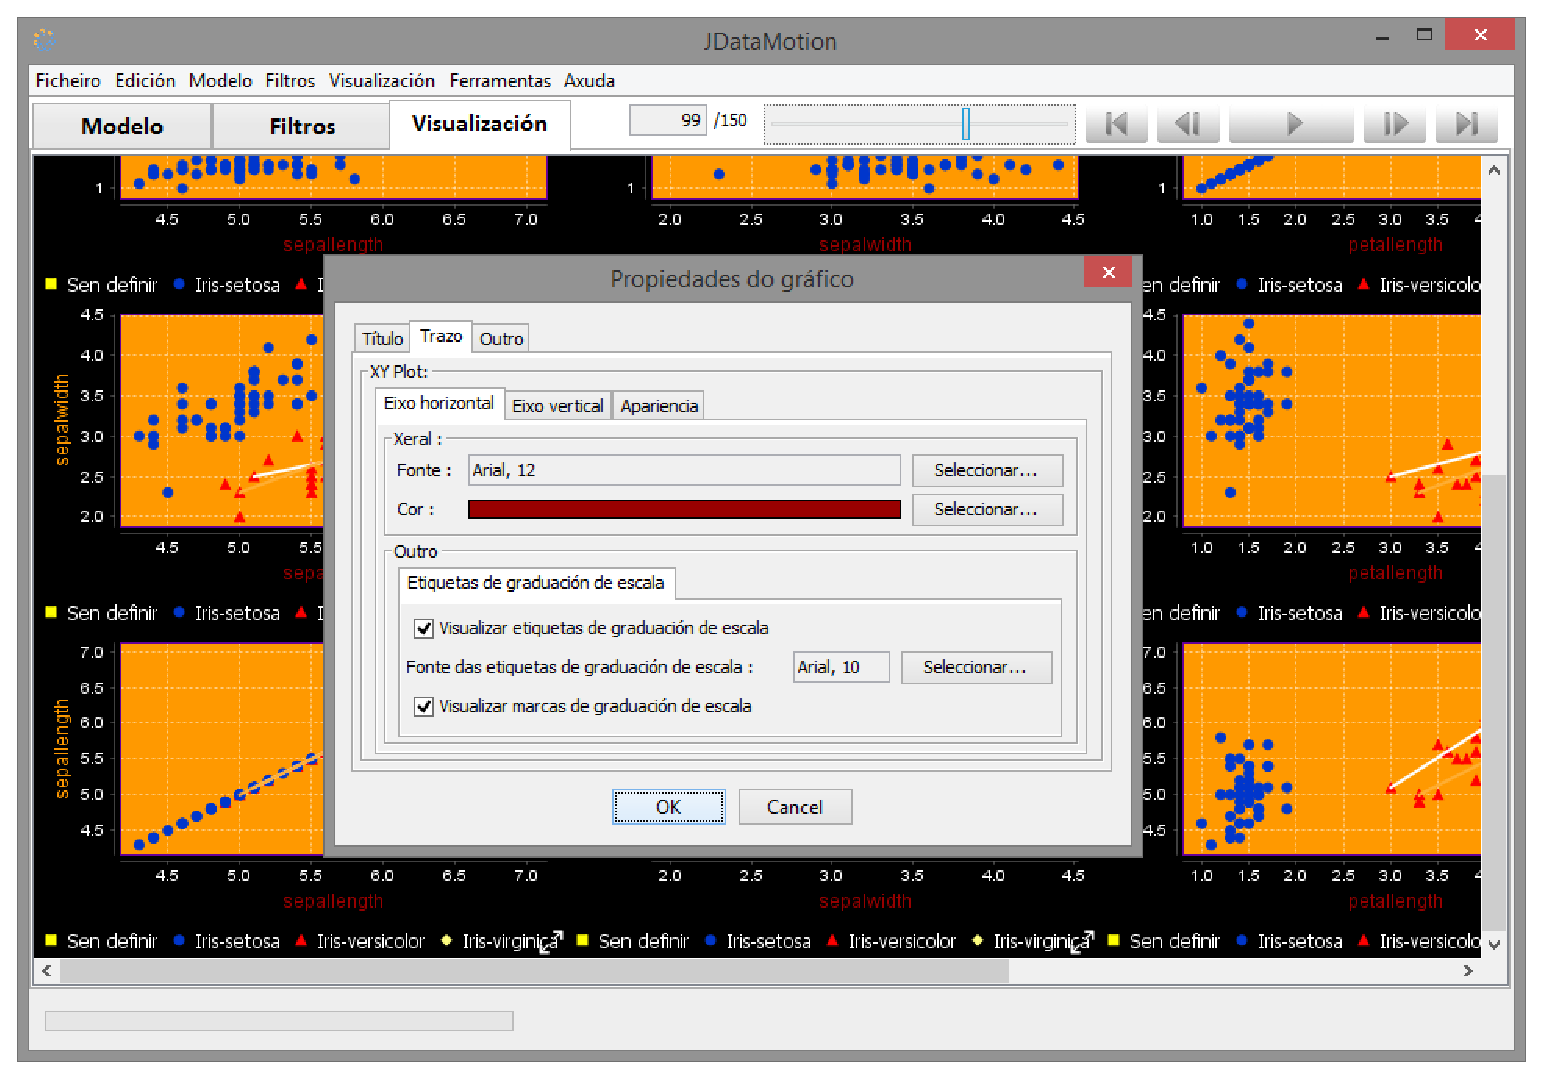
\includegraphics[width=\textwidth,height=\textheight,keepaspectratio]{figuras/RF32}
\caption{Comprobación heurística do RF32}
\label{RF32}
\end{figure}
\item[Resultado]
Correcto.
\end{description}

\subsection{Requisitos de calidade}

\subsubsection*{RC01}
\begin{description}
\item[Título] \hfill
Latencia mínima para o procesamento
\item[Descrición] \hfill
A aplicación debe responder nun tempo razoable ás operacións executadas polo usuario, e intentar que esa latencia escale de xeito controlado ao aumentar a talla dos parámetros.
\item[Importancia] \hfill
Esencial
\item[Tipo de proba] \hfill
Avaliación de prestacións
\item[Descrición]
Preparamos 16 ficheiros ARFF de datos, con 11, 22, 33 e 44 atributos, e 2500, 5000, 7500 e 10000 instancias, cubrindo todas as combinacións. Executamos estos ficheiros activando a bandeira Controlador.DEBUG para obter os tempos de execución das tres rexións que compoñen o refresco (a operación máis custosa do programa). En concreto, tomaremos individualmente o tempo que tarda en refrescar cada menú (Modelo, Filtros e Visualización coa matriz de diagramas de dispersión completa). O de filtros descartarémolo xa que a súa latencia é insignificante e non aumenta coa talla do arquivo. Os resultados obtidos foron os seguintes:
\begin{figure}
\centering
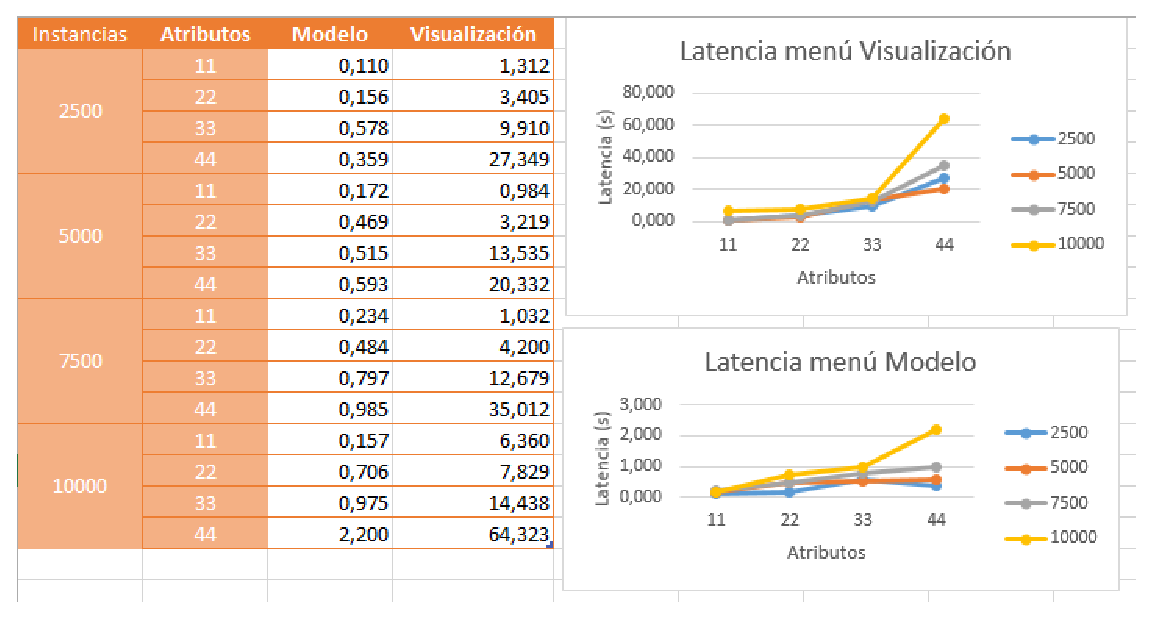
\includegraphics[width=\textwidth,height=\textheight,keepaspectratio]{figuras/eficiencia}
\caption{Comprobación prestacións do RC01}
\label{eficiencia}
\end{figure}
A latencia vólvese crítica no refresco do menú de visualización, e a escalabilidade empeora co aumento do número de atributos. O Modelo sen embargo escala relativamente mellor con respecto a instancias e atributos. Cabe destacar que é ata certo punto razonable que o menú de Visualización escale tan mal, pois sufre os aumentos no número de atributos ao cadrado (a matriz de diagramas ten n*n elementos).
\item[Resultado]
Aceptable.
\end{description}

\subsection{Requisitos de deseño}

\subsubsection*{RD01}
\begin{description}
\item[Título] \hfill
Modularidade no deseño dos filtros
\item[Descrición] \hfill
A aplicación debe facilitar unha interface para a inclusión e uso de filtros personalizados por parte de calquera desenvolvedor de software que a implemente dentro do proxecto.
\item[Importancia] \hfill
Esencial
\item[Tipo de proba] \hfill
Avaliación heurística
\item[Descrición]
O diagrama de deseño exposto neste documento da fe de que se cumpleu este requisito. De todos xeitos pódese probar a nivel de implementación importando un filtro dende JAR.
\item[Resultado]
Correcto.
\end{description}

\subsection{Requisitos non funcionais}

\subsubsection*{RNF01}
\begin{description}
\item[Título] \hfill
Formatos de arquivo admitidos ao importar e exportar arquivos
\item[Descrición] \hfill
A aplicación debe estar preparada para importar e exportar arquivos en distintos formatos, como son o CSV e ARFF.
\item[Importancia] \hfill
Esencial
\item[Tipo de proba] \hfill
Test implementado en JUnit.
\item[Descrición]
Xa foi comprobado no TestRF01\_1 e TestRF01\_2
\item[Resultado]
Correcto.
\end{description}

\subsubsection*{RNF02}
\begin{description}
\item[Título] \hfill
Relación programa-sesión
\item[Descrición] \hfill
Cada instancia do programa debe traballar cunha única sesión (experimento).
\item[Importancia] \hfill
Esencial
\item[Tipo de proba] \hfill
Test implementado en JUnit.
\item[Descrición]
Xa foi comprobado no TestRF0304, xa que ao abrir unha nova sesión perdíase a anterior
\item[Resultado]
Correcto.
\end{description}

\subsubsection*{RNF03}
\begin{description}
\item[Título] \hfill
Implementación en Java
\item[Descrición] \hfill
O software tense que desenvolver na linguaxe de programación Java.
\item[Importancia] \hfill
Esencial
\item[Tipo de proba] \hfill
Avaliación heurística
\item[Descrición]
Podemos comprobalo simplemente accedendo ao código fonte do proxecto.
\item[Resultado]
Correcto.
\end{description}

\subsubsection*{RNF04}
\begin{description}
\item[Título] \hfill
Representación matricial dos diagramas de dispersión
\item[Descrición] \hfill
Os diagramas de dispersión represéntanse de xeito matricial, facendo que cada parámetro dentro dun eixo sexa enfrontado a cada un dos demais do outro eixo, e en cada punto desa dupla se sitúe o diagrama de dispersión que compara ambos parámetros. Deste xeito, os diagramas de dispersión non son acumulables: se temos un que representa X (abscisas) fronte a Y (ordenadas), non podemos engadir outro que represente X (abscisas) fronte a Y (ordenadas), pois ocuparían ambos a mesma cela dentro da matriz de diagramas de dispersión.
\item[Importancia] \hfill
Esencial
\item[Tipo de proba] \hfill
Test implementado en JUnit.
\item[Descrición]
Xa foi comprobado na avaliación heurística de RF11.
\item[Resultado]
Correcto.
\end{description}

\subsubsection*{RNF05}
\begin{description}
\item[Título] \hfill
Entrega dentro de prazo
\item[Descrición] \hfill
Débese entregar unha versión funcional e documentada antes do día 10 de Xullo de 2015, ás 14:00 horas, pois é o momento no que remata o prazo de entrega.
\item[Importancia] \hfill
Esencial
\end{description}

A matriz de trazabilidade que relacionaría cada requisito cun tipo de proba (heurística ou test en JUnit) é a que se presenta a continuación:

\begin{sidewaysfigure}[ht]
\includegraphics[width=\textwidth,height=\textheight,keepaspectratio]{figuras/trazabilidade}
\caption{Matriz de trazabilidade}
\label{trazabilidade}
\end{sidewaysfigure}
